\documentclass[letterpaper,12pt]{report}

\usepackage[english]{babel}
\usepackage[a4paper,left=1in,right=1in,top=1in,bottom=1in]{geometry}
\usepackage[nodisplayskipstretch]{setspace}
\usepackage[fleqn]{amsmath}
\usepackage{amssymb}
\usepackage{url}
\usepackage{verbatim}
\usepackage[title]{appendix}
\usepackage{indentfirst}
\usepackage{booktabs}
\usepackage{multirow}
\usepackage{ragged2e}
\setlength{\RaggedRightParindent}{\parindent}
\usepackage{upgreek}
\usepackage{gensymb}
\usepackage[T1]{fontenc}
\usepackage[titles]{tocloft}
\renewcommand{\cftchapleader}{\cftdotfill{\cftdotsep}} % Force chapters to have dot fill
\usepackage{xspace}
% xcolor allows rowcolors for tables
\usepackage[table,x11names,dvipsnames,table]{xcolor}
% \usepackage[usenames]{color}
\usepackage{ifthen}
\usepackage{cancel}
\usepackage{array}
\usepackage{tabulary}
\usepackage{authblk}
\usepackage{tikz}
\usepackage{pdflscape}
\usepackage[normalem]{ulem}
\usepackage{longtable}
\usepackage[utf8]{inputenc}
\usepackage[scientific-notation=true]{siunitx}
\usepackage{pdfpages}

% Set up color palettes 
\definecolor{pgreen}     {RGB}{50,162,81}
\definecolor{porange}    {RGB}{255,127,15}
\definecolor{pblue}      {RGB}{60,183,204}
\definecolor{pyellow}    {RGB}{255,217,74}
\definecolor{pteal}      {RGB}{57,115,124}
\definecolor{pauburn}    {RGB}{184,90,13}
\definecolor{mygray}{gray}{0.9}

\usepackage{hyperref}
\hypersetup{pdfborder={0 0 0},
            % colorlinks=true,
            colorlinks=false,
            % urlcolor=porange,
            % linkcolor=pauburn,
            % linkcolor=pauburn,
            % citecolor=pteal
            }

\usepackage[capitalize]{cleveref}
\newcommand{\crefrangeconjunction}{--}

% Set up line numbering; using lineno to number lines of paragraphs with
% equations sanely
\usepackage[right, mathlines]{lineno}
\setlength\linenumbersep{1cm}
\def\linenumberfont{\normalfont\scriptsize\sffamily}

% Set up caption formatting
\usepackage{subcaption}
\usepackage[format=plain, labelsep=period, singlelinecheck=true, skip=2pt, font=sf]{caption}
\DeclareCaptionLabelFormat{noSpace}{{#1}{#2}}
\DeclareCaptionListFormat{figList}{{#2}.}
\DeclareCaptionListFormat{sFigList}{Figure S{#2}.}

%%%%%%%%%%%%%%%%%%%%%%%%%%%%%%%%%%%%%%%%%%%%%%%%%%%%%%%%%%%%%%%%%%%%%%%%%%%%%%%%
% % Define tightly formated list environments via enumitem
\usepackage{enumitem}
\newenvironment{tightItemize}{%
\begin{itemize}[noitemsep, topsep=0pt, parsep=0pt, partopsep=0pt]}
{\end{itemize}}

\newenvironment{veryTightItemize}{%
\begin{itemize}[noitemsep, topsep=0pt, parsep=0pt, partopsep=0pt, leftmargin=*]}
{\end{itemize}}

\newenvironment{tightEnumerate}{%
\begin{enumerate}[noitemsep, topsep=0pt, parsep=0pt, partopsep=0pt]}
{\end{enumerate}}

\newenvironment{veryTightEnumerate}{%
\begin{enumerate}[noitemsep, topsep=0pt, parsep=0pt, partopsep=0pt, leftmargin=*]}
{\end{enumerate}}

% Redefine abstract environment as a list to control left/right margins
% From https://tex.stackexchange.com/a/151589
\renewenvironment{abstract}
 {\small
  \begin{center}
  \bfseries \abstractname\vspace{-.5em}\vspace{0pt}
  \end{center}
  \list{}{%
    \setlength{\leftmargin}{5mm}%
    \setlength{\rightmargin}{\leftmargin}%
  }%
  \item\relax}
 {\endlist}

\newcommand{\citationNeeded}{\textcolor{magenta}{\textbf{[CITATION NEEDED!]}}\xspace}
\newcommand{\tableNeeded}{\textcolor{magenta}{\textbf{[TABLE NEEDED!]}}\xspace}
\newcommand{\figureNeeded}{\textcolor{magenta}{\textbf{[FIGURE NEEDED!]}}\xspace}
\newcommand{\highLight}[1]{\textcolor{magenta}{\MakeUppercase{#1}}}
\newcommand{\figtitle}[1]{\textbf{#1}}

\newcommand{\datasets}{data sets\xspace}
\newcommand{\dataset}{data set\xspace}

\newcommand{\editorialNote}[1]{\textcolor{red}{[\textit{#1}]}}
\newcommand{\ignore}[1]{}
\newcommand{\addTail}[1]{\textit{#1}.---}
\newcommand{\super}[1]{\ensuremath{^{\textrm{#1}}}}
\newcommand{\sub}[1]{\ensuremath{_{\textrm{#1}}}}
\newcommand{\dC}{\ensuremath{^\circ{\textrm{C}}}}
\newcommand{\tb}{\hspace{2em}}
\newcommand{\tn}{\tabularnewline}
\newcommand{\spp}[1]{\textit{#1}}

\providecommand{\e}[1]{\ensuremath{\times 10^{#1}}}

\newcommand{\change}[2]{{\color{red} #2}\xspace}
\newcommand{\thought}[1]{\textcolor{purple}{THOUGHT: #1}}

\newcommand{\widthFigure}[6]{\begin{figure}[htbp]
\begin{center}
    \includegraphics[width=#1\textwidth]{#2}
    \captionsetup{#3}
    \caption[#4]{#5}
    \label{#6}
    \end{center}
    \end{figure}}

\newcommand{\heightFigure}[6]{\begin{figure}[htbp]
\begin{center}
    \includegraphics[height=#1\textheight]{#2}
    \captionsetup{#3}
    \caption[#4]{#5}
    \label{#6}
    \end{center}
    \end{figure}}

\newcommand{\smartFigure}[5]{%
    \begin{figure}[htbp]
        \begin{center}
            \includegraphics[width=\textwidth,height=0.95\textheight,keepaspectratio]{#1}
            \captionsetup{#2}
            \caption[#3]{#4}
            \label{#5}
        \end{center}
    \end{figure}
}

\newcommand{\mFigure}[4]{\smartFigure{#1}{listformat=figList}{#2}{#3}{#4}\clearpage}
\newcommand{\embedHeightFigure}[5]{\heightFigure{#1}{#2}{listformat=figList}{#3}{#4}{#5}}
\newcommand{\embedWidthFigure}[5]{\widthFigure{#1}{#2}{listformat=figList}{#3}{#4}{#5}}
\newcommand{\siFigure}[4]{\smartFigure{#1}{name=Figure S, labelformat=noSpace, listformat=sFigList}{#2}{#3}{#4}\clearpage}


%% macro to make long strings breakable over lines
\makeatletter
\def\breakable#1{\xHyphen@te#1$\unskip}
\def\xHyphen@te{\@ifnextchar${\@gobble}{\sw@p{\allowbreak{}\xHyphen@te}}}
% \def\xHyphen@te{\@ifnextchar${\@gobble}{\sw@p{\hskip 0pt plus 1pt\xHyphen@te}}}
\def\sw@p#1#2{#2#1}
\makeatother


\newcommand{\makeSampleTable}[3]{
\begin{longtable}{lllll}
  \caption{#1} \label{table:#2} \\
  
  \hline 
  \multicolumn{1}{c}{Sample ID} & 
  \multicolumn{1}{c}{Species} & 
  \multicolumn{1}{c}{Latitude} & 
  \multicolumn{1}{c}{Longitude} & 
  \multicolumn{1}{c}{Passed Filtering} \\ 
  \hline 
  \endfirsthead
  
  \multicolumn{4}{c}%
  {{\tablename\ \thetable{} -- continued from previous page}} \\
  
  \hline 
  \multicolumn{1}{c}{Sample ID} & 
  \multicolumn{1}{c} {Species} & 
  \multicolumn{1}{c} {Latitude} & 
  \multicolumn{1}{c} {Longitude} & 
  \multicolumn{1}{c} {Passed Filtering} \\ 
  \hline 
  \endhead
  
  \hline \multicolumn{4}{r}{{Continued on next page}} \\
  \endfoot
  
  \hline 
  % \hline
  \endlastfoot
  
  \input{#3}
\end{longtable}
\clearpage

}


\newcommand{\makePhyloSampleTable}[3]{
\begin{longtable}{llllllll}
  \caption{#1} \label{#2} \\
  
  \hline 
  \multicolumn{1}{c}{ID} &
  \multicolumn{1}{c}{Sample ID} & 
  \multicolumn{1}{c}{Species} & 
  \multicolumn{1}{c}{Latitude} & 
  \multicolumn{1}{c}{Longitude} & 
  \multicolumn{1}{c}{Passed Filtering} & 
  \multicolumn{1}{c}{Phycoeval} & 
  \multicolumn{1}{c}{Structure} \\ 
  \hline 
  \endfirsthead
  
  \multicolumn{4}{c}%
  {{\tablename\ \thetable{} -- continued from previous page}} \\
  
  \hline 
  \multicolumn{1}{c}{ID} &
  \multicolumn{1}{c}{Sample ID} & 
  \multicolumn{1}{c}{Species} & 
  \multicolumn{1}{c}{Latitude} & 
  \multicolumn{1}{c}{Longitude} & 
  \multicolumn{1}{c}{Passed Filtering} & 
  \multicolumn{1}{c}{Phycoeval} & 
  \multicolumn{1}{c}{Structure} \\ 
  \hline 
  \endhead
  
  \hline \multicolumn{4}{r}{{Continued on next page}} \\
  \endfoot
  
  \hline 
  % \hline
  \endlastfoot
  
  \input{#3}
\end{longtable}
\clearpage

}
\newcommand{\given}{\ensuremath{\,|\,}\xspace}
\newcommand{\pr}{\ensuremath{p}}

\newcommand{\fst}{$F_{st}$\xspace}
\newcommand{\ul}{\microL\xspace}
\newcommand{\um}{\microM\xspace}

\newcommand{\amer}{\textit{A. americanus}\xspace}
\newcommand{\terr}{\textit{A. terrestris}\xspace}
\newcommand{\adegenet}{\textit{adegenet}\xspace}
\newcommand{\structure}{\textit{STRUCTURE}\xspace}
\newcommand{\pophelper}{\textit{POPHELPER}\xspace}
\newcommand{\stacks}{\textit{Stacks}\xspace}
\newcommand{\processradtags}{\textit{process\_radtags}\xspace}
\newcommand{\populations}{\textit{populations}\xspace}
\newcommand{\clonefilter}{\textit{clone\_filter}\xspace}
\newcommand{\bgcutils}{\textit{bgc\_utils}\xspace}
\newcommand{\bgc}{\textit{BGC}\xspace}
\newcommand{\vcftools}{\textit{VCFtools}\xspace}
\newcommand{\matplotlib}{\textit{Matplotlib}\xspace}

\newcommand{\ecoevolity}{\textit{ecoevolity}\xspace}
\newcommand{\Ecoevolity}{\textit{Ecoevolity}\xspace}
\newcommand{\beast}{\textit{StarBEAST2}\xspace}
\newcommand{\beastcore}{\textit{BEAST2}\xspace}
\newcommand{\dendropy}{\textit{DendroPy}\xspace}
\newcommand{\seqgen}{\textit{Seq-Gen}\xspace}
\newcommand{\python}{\textit{Python}\xspace}




\newcommand{\allsites}{all sites\xspace}
\newcommand{\snps}{SNPs\xspace}
\newcommand{\noerrors}{No errors}
\newcommand{\singletoneighty}{20\% singleton errors}
\newcommand{\singletonsixty}{40\% singleton errors}
\newcommand{\heteighty}{20\% het errors}
\newcommand{\hetsixty}{40\% het errors}


\newcommand{\data}{\ensuremath{D}\xspace}
\newcommand{\model}[1][]{\ensuremath{M_{#1}}\xspace}
\newcommand{\parameters}[1][]{\ensuremath{\Theta_{#1}}\xspace}
\newcommand{\parameter}[1][]{\ensuremath{\theta_{#1}}\xspace}
\newcommand{\diff}[1]{\ensuremath{\mathrm{d}#1}}

\newcommand{\distgamma}{\ensuremath{\textrm{Gamma}}\xspace}
\newcommand{\distexponential}{\ensuremath{\textrm{Exponential}}\xspace}
\newcommand{\dgamma}[2]{\ensuremath{\distgamma(\textrm{shape} = #1, \textrm{mean} = #2)}}
\newcommand{\dexponential}[1]{\ensuremath{\distexponential(\textrm{mean} = #1)}}
\newcommand{\gshape}{\ensuremath{k}\xspace}
\newcommand{\gscale}{\ensuremath{\theta}\xspace}

\newcommand{\nloci}[1][]{\ensuremath{m_{#1}\xspace}}

\newcommand{\observedallelecount}[1][]{\ensuremath{n_{#1}}\xspace}
\newcommand{\observedredallelecount}[1][]{\ensuremath{r_{#1}}\xspace}

\newcommand{\nodeallelecount}[2]{\ensuremath{n_{#1}^{#2}}}
\newcommand{\noderedallelecount}[2]{\ensuremath{r_{#1}^{#2}}}

\newcommand{\allelecount}[1][]{\ensuremath{\nodeallelecount{#1}{}}\xspace}
\newcommand{\redallelecount}[1][]{\ensuremath{\noderedallelecount{#1}{}}\xspace}

\newcommand{\leafallelecounts}[1][]{\ensuremath{\mathbf{n}_{#1}}\xspace}
\newcommand{\leafredallelecounts}[1][]{\ensuremath{\mathbf{r}_{#1}}\xspace}
\newcommand{\maxleafallelecounts}{\ensuremath{\textrm{max}(\mathbf{n})}\xspace}

\newcommand{\comparisondata}[1][]{\ensuremath{D_{#1}}\xspace}
\newcommand{\alldata}[1][]{\ensuremath{\mathbf{D}}\xspace}

\newcommand{\branchindex}{\ensuremath{x}\xspace}
\newcommand{\allelecountbottom}[1][\branchindex]{\nodeallelecount{#1}{B}}
\newcommand{\allelecounttop}[1][\branchindex]{\nodeallelecount{#1}{T}}
\newcommand{\redallelecountbottom}[1][\branchindex]{\noderedallelecount{#1}{B}}
\newcommand{\redallelecounttop}[1][\branchindex]{\noderedallelecount{#1}{T}}

\newcommand{\rgmurate}{\ensuremath{u}\xspace}
\newcommand{\grmurate}{\ensuremath{v}\xspace}
\newcommand{\murate}[1][]{\ensuremath{\mu_{#1}}\xspace}
\newcommand{\murates}[1][]{\ensuremath{\boldsymbol{\mu}_{#1}}\xspace}
\newcommand{\gfreq}[1][]{\ensuremath{\pi_{#1}}\xspace}
\newcommand{\gfreqs}[1][]{\ensuremath{\boldsymbol{\pi}_{#1}}\xspace}

\newcommand{\genetree}[1][]{\ensuremath{g_{#1}}\xspace}
\newcommand{\sptree}[1][]{\ensuremath{S_{#1}}\xspace}
\newcommand{\sptrees}[1][]{\ensuremath{\mathbf{S}_{#1}}\xspace}

\newcommand{\divtime}[1][]{\ensuremath{\tau_{#1}}\xspace}
\newcommand{\descendantpopindex}[1]{\ensuremath{D{#1}}}
\newcommand{\rootpopindex}[1][]{\ensuremath{R{#1}}\xspace}
\newcommand{\epopsize}[1][]{\ensuremath{N_{e}^{#1}}\xspace}
\newcommand{\rootpopsize}{\epopsize[\rootpopindex]\xspace}
\newcommand{\tippopsize}[1][]{\epopsize[\descendantpopindex{#1}]\xspace}

% Fig reference with parentheses
\newcommand{\mainfigsp}{(\cref{fig:time1000,fig:time500,fig:time250,fig:roottheta1000,fig:roottheta500,fig:roottheta250,fig:theta1000,fig:theta500,fig:theta250})}
\newcommand{\timefigsp}{(\cref{fig:time1000,fig:time500,fig:time250})}
\newcommand{\thetafigsp}{(\cref{fig:theta1000,fig:theta500,fig:theta250})}
\newcommand{\rootfigsp}{(\cref{fig:roottheta1000,fig:roottheta500,fig:roottheta250})}

% Fig references without parentheses
\newcommand{\mainfigs}{\cref{fig:time1000,fig:time500,fig:time250,fig:roottheta1000,fig:roottheta500,fig:roottheta250,fig:theta1000,fig:theta500,fig:theta250}}
\newcommand{\timefigs}{\cref{fig:time1000,fig:time500,fig:time250}}
\newcommand{\thetafigs}{\cref{fig:theta1000,fig:theta500,fig:theta250}}
\newcommand{\rootfigs}{\cref{fig:roottheta1000,fig:roottheta500,fig:roottheta250}}

\newcommand{\uL}{$\mu$L}
\newcommand{\uM}{$\mu$M}

% References
\usepackage[backend=biber, style=apa, sorting=nyt, refsection=chapter]{biblatex}
\addbibresource{~/Documents/library.bib}
\addbibresource{bib/references.bib}
% \addbibresource{bib/kac_zotero.bib}

% Graphics
\usepackage{graphicx}
\graphicspath{
  {../sims/plots-tex/}
  {../toad-evolution/structure/plots}
  {../toad-evolution/maps/out}
  {../toad-evolution/pca/out-plots}
  {../toad-evolution/iqtree}
  {../toad-evolution/dsuite}
  {../toad-evolution/plots-tex}
  {../toad-evolution/bgc/out-popmap2-95}
  {../toad-evolution/phycoevol}
}

% Manuscript %%%%%%%%%%%%%%%%%%%%%%%%%%%%%%%%%%%%%%%%%%%%
\doublespacing
\begin{document}

% \clearpage
% \thispagestyle{empty}
% 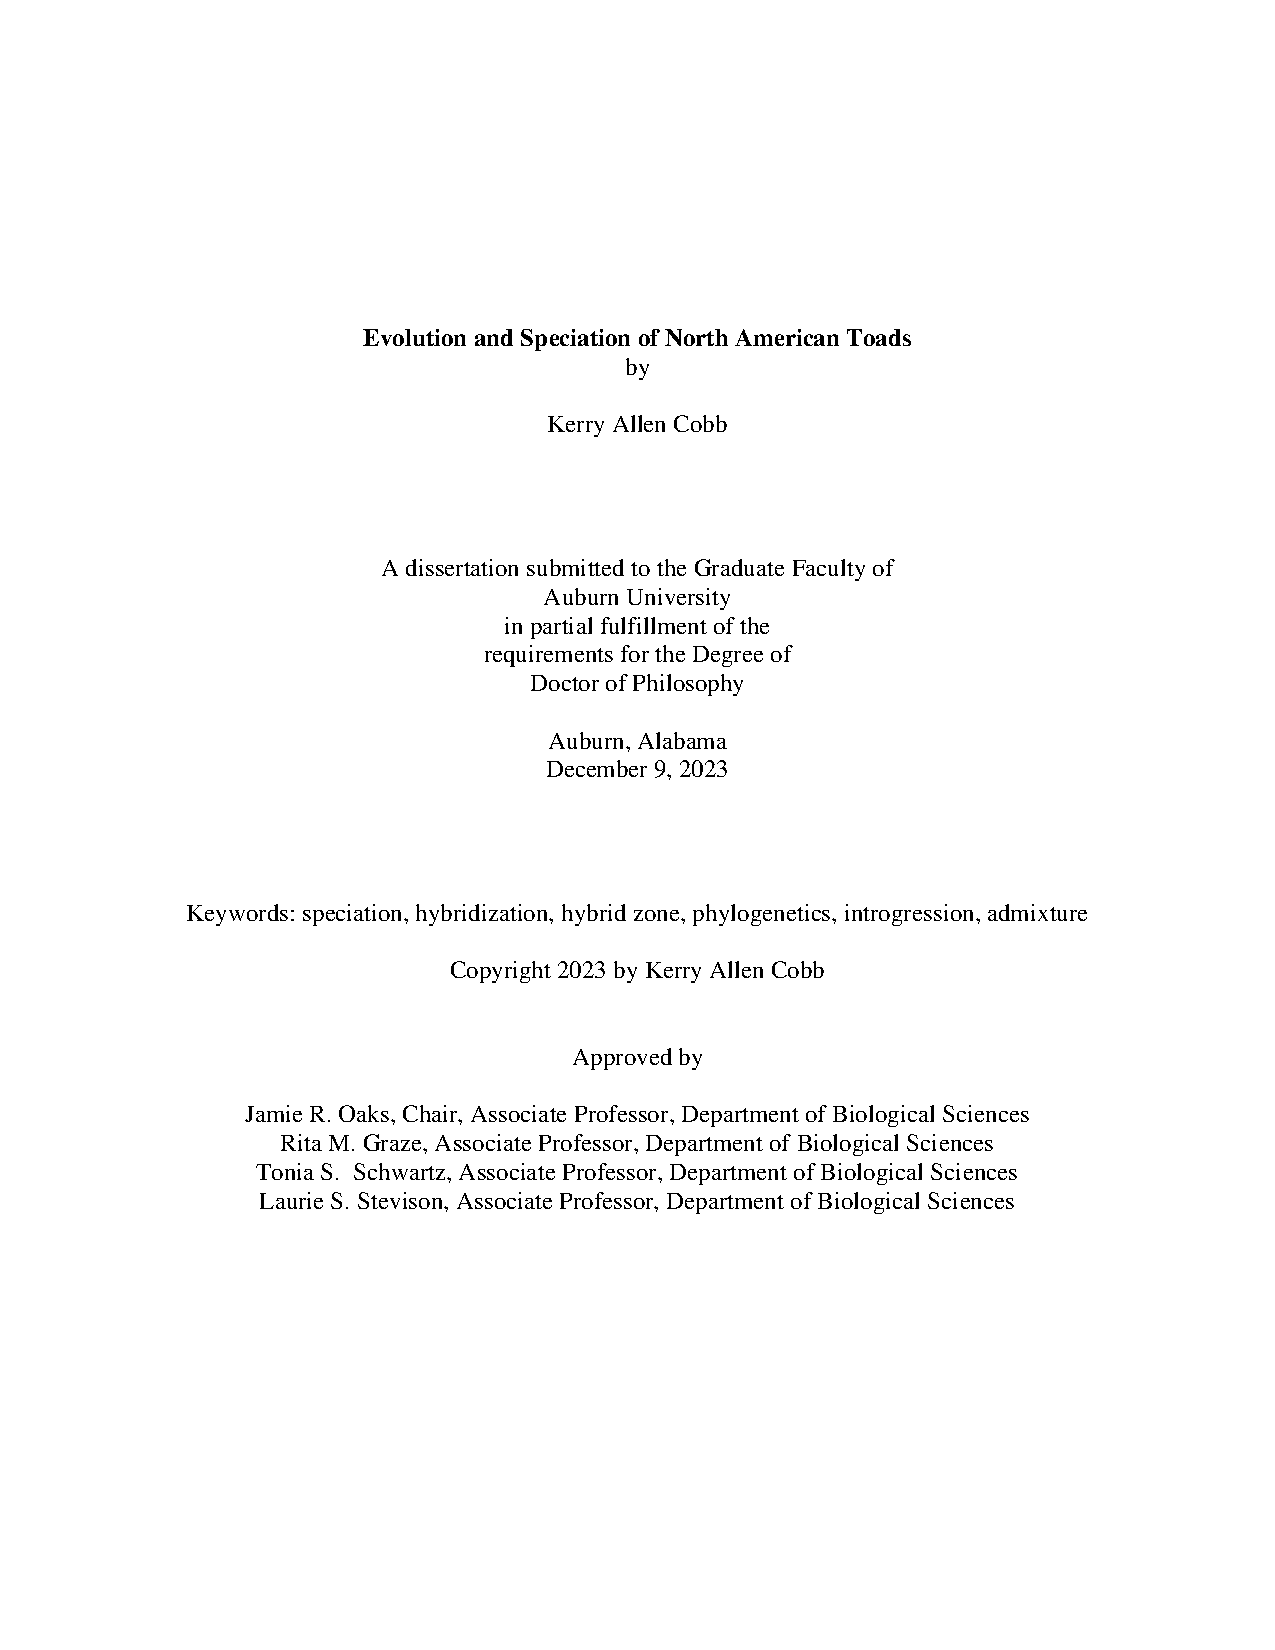
\includepdf{sections/title-page.pdf}

\begin{linenumbers}

% \chapter*{Abstract}
\ldots
% \addcontentsline{toc}{chapter}{Abstract}

% \chapter*{Acknowledgments}

I would like to express my deep appreciation to the individuals who have played 
pivotal roles leading to the successful completion of my PhD dissertation. 
Their support, encouragement, and guidance have been instrumental in 
shaping my academic journey.
First and foremost, I am grateful to my advisor Jamie Oaks for his 
generosity, kindness, and mentorship throughout my time at Auburn. 
You have been a wonderful teacher and a fantastic role model. 
I would also like to thank my committee member Laurie Stevison for your 
advice and words of encouragement. And thank you to my other committee members
Tonia Schwartz and Rita Graze for your valuable input and expertise. 
To my dear friend and labmate, Randy Klabacka, I will always cherish the fond 
memories we created and the enlightening conversations that we've had during our time at Auburn. 
I would also like to acknowledge my other labmates, Matt Buehler,
Saman Jahangiri, Tanner Meyers, Morgan Muell, Claire Tracy, J.R. Wood, 
for making my time at Auburn an enjoyable and enriching experience. 
The stimulating environment created by all of you along with your camaraderie, 
have made my time at Auburn an incredibly enriching and enjoyable experience.
To my parents Mark and Jane and my sister Claire, I am immensely grateful for 
the love, support, and encouragement you have provided me throughout my life. 
I also thank you Mom and Dad for fostering my curiosity for the natural world
from a young age, for being wonderful role models, and for making education
a high priority in my upbringing. 
Lastly, I want to thank my wonderful wife, Aura Cobb, for her unwavering support, love, 
and patience and for the sacrifices you have made for me to accomplish this dream. 
I am profoundly grateful to have you in my life and to have had you by my side 
during this endeavor. 
% \addcontentsline{toc}{chapter}{Acknowledgedments}

\tableofcontents
\addcontentsline{toc}{chapter}{Table of Contents}

\listoffigures
\addcontentsline{toc}{chapter}{List of Figures}

\listoftables
\addcontentsline{toc}{chapter}{List of Tables}

% \chapter{Introduction}
% 
% Introduction
Speciation is the driving force behind the incredible diversity of life on Earth. 
By studying this process, we gain insights into the mechanisms that 
have shaped the natural world, enabling us to appreciate and understand this 
biodiversity.
A fundamental aspect of speciation is the evolution of reproductive isolation.
This phenomenon has puzzled and captivated evolutionary biologists since the 
field's inception \parencite{mallet2008}.
Reproductive isolation was first viewed as incompatible with evolution by  
natural selection as it was inconceivable how natural selection might produce 
such an outcome \parencite{mallet2008}.
It is now appreciated that reproductive isolation is in fact compatible with 
evolution by natural selection, but mysteries abound \parencite{coyne2004}.
Why do organisms form discrete clusters instead of existing on a continuum?
What evolutionary processes drive reproductive isolation?
Which genes are involved and what are their functions under normal circumstances?
What are the targets of selection that drive evolution of these genes? 
What is the role of gene flow in the speciation process?
With increasingly powerful tools at their disposal, biologists are directing  
more attention than ever before into seeking answers to these questions.

% Toads
Toads in the family Bufonidae have held a prominent place in the speciation 
literature \parencite{blair1972}.
They have a number of qualities that makes them attractive for furthering our
understanding of the speciation process. 
Among these qualities is the ease with which the primary behavioral isolating mechanisms, 
spawning period and advertisement call, can be measured and quantified in order 
to understand the strength of prezygotic mating barriers and possible patterns 
consistent with reinforcement \parencite{cocroft1995,blair1974,kennedy1962}.
Researchers in the past were also drawn by the ease with which they can be 
crossed in the laboratory \parencite{blair1972}.
Spawning can be induced hormonally or performed in vitro, facilitating the planning  
and execution of experiments \parencite{trudeau2010}.
The females of many species can produce thousands of offspring which are externally 
fertilized making a variety of embryological observations or manipulations possible \parencite{blair1972}.
Many species pairs have proven to be reproductively compatible through laboratory crosses \parencite{blair1972}. 
This has provided an opportunity to investigate the tempo of the evolution of 
reproductive incompatibility and to understand the importance of pre-mating 
barriers \parencite{sasa1998,malone2008,fontenot2011}.
Another attractive quality of Bufonidae is the existence of several known 
hybrid zones which provide useful opportunities for studying the evolution 
of reproductive isolation in a natural setting \parencite{green1996,vanriemsdijk2023}. 

Unlike many organisms which have been the subject of intensive study in the 
context of speciation, such as \textit{Drosophila}, \textit{Mus}, and \textit{Heliconius},
most Bufonidae have homomorphic sex chromosomes \parencite{blair1972}.
This is an interesting contrast in light of the apparent importance of sex chromosomes
in the evolution of reproductive incompatibility and 
the roll of heterogamety in explaining evolutionary patterns such as Haldane's 
rule, faster male evolution, and faster-X evolution \parencite{delph2016}. 
Furthermore, there is evidence of sex chromosome turnovers within Bufonidae
which presents an opportunity to study differences in the evolution of  
reproductive incompatibility among closely related species with different 
sex determination systems \parencite{dufresnes2020,stock2011}. 
All of these qualities, along with a near global distribution and large diversity 
of species (642 species; \cite{amphibiaweb2023}) and ecological niches, make Bufonidae 
an excellent group to further our understanding of the evolution of reproductive 
incompatibility.



% Hybridization usefulness
In the first chapter of my dissertation I investigate a putative hybrid zone between 
\textit{Anaxyrus americanus} and \textit{A. terrestris}, two species in 
the family Bufonidae. 
Hybrid zones are increasingly appreciated to be a widespread phenomenon in nature.
One that can have important evolutionary consequences when it comes to the
process of speciation \parencite{moran2021}.
Hybrid zones also present a valuable opportunity to investigate reproductive 
incompatibility \parencite{rieseberg1999}. 
The production of large numbers of recombinant offspring through multiple 
generations of backcrossing under natural conditions cannot be achieved
through captive breeding for most organisms.

The only prior evidence of hybridization between \amer and \terr comes from anecdotal reports
and a single study of morphological variation across the contact zone between
these two species in central Alabama \parencite{mount1975,weatherby1982}. 
The amount of introgression, if any, within this putative hybrid zone is unknown.
Using genome-wide data collected from a large sample across the hybrid zone, 
I characterize introgression between these two species for the first time.  
I find that introgression between them is extensive and I identify many 
candidate loci that may be involved in reproductive incompatibility.
This study can serve as a guide to future studies in this system which could 
leverage quantitative measures of prezygotic isolation such 
as calls and breeding period, reference genomes, or crossing experiments paired
with cutting edge genomic tools such as CRISPR-Cas9 to shed light on the process
of speciation. 
In combination with other toad hybrid zones, there is a great deal we could 
learn about whether there are recurrent patterns in toad speciation, with
their homomorphic sex chromosomes are a useful contrast against other taxa.

% Evolutionary history
Hybrid zones have great potential for furthering our understanding of speciation.
However, they provide only a snapshot in time. 
There is a great deal of historical context that is also important to understand. 
Questions such as, how long has it been since hybridizing species have diverged?
What are the environmental factors that drive divergence between them? 
And, what are the lasting consequences of hybridization?
In the second chapter of my dissertation, I investigate the evolutionary history of 
species within the genus \anaxyrus to attempt to answer these questions. 
To accomplish this, I infer the phylogenetic relationships among species in this genus
from genome-wide sequence data and estimate the divergence times for nodes in 
the phylogenetic tree. 
I also test for a history of admixture to understand the importance of 
historical introgression among ancestral species during the evolutionary history of the genus.

To try to understand what factors might play a role in driving divergence
between populations and potentially result in speciation, I also investigate 
population structure within several species.
The relationships and divergence-time estimates that I infer from the genomic 
data differ substantially from previous studies based on more limited data
and methods \parencite{fontenot2011,graybeal1997,masta2002,pramuk2007,pyron2011,portik2023}.
I also find evidence of previously unrecognized hybridization in the past and 
present between species of \anaxyrus which reinforces the increasingly appreciated 
recognition of gene flow as a common and important process during the 
diversification of organisms.
My analysis of population structure shows strong population differentiation
in one species which could be in the early stage of speciation. 
This chapter highlights the utility of \anaxyrus for understanding speciation
as there is potentially hybridization occurring at multiple stages of the 
speciation process. 

% Methods
The inferences made about the evolutionary process in the previous two chapters
rely heavily on a suite of computational methods developed for the task. 
All of these methods make assumptions about the processes that produce the 
data, i.e. DNA sequences, which are used as input. 
These are often simplifying assumptions made to achieve tractable models and 
computation, many of which are known to be violated.
Many simplifying assumptions are sure to be violated and we know this to be the case for many of them.
Other assumptions are made because they reflect our best set of beliefs about 
the evolutionary process or because work has not yet been done to incorporate 
additional complexity into the methods. 
Many of these are sure to be violated as well but are more challenging to
recognize.
Violations of assumptions may not be highly problematic \parencite{oaks2020},
but the impact of many violations have never been evaluated. 
In the third chapter of my dissertation, I investigate the impact of 
errors and biases that can arise through the collection and processing DNA sequence data.
I find that these violations have a modest impact on inference. 
When clustering reads to construct an alignment, it is necessary to set a minimum  
similarity threshold that will very likely exclude variants from the alignment. 
In simulated data, I found this type of data acquisition bias had the effect of
underestimating recent divergence times and underestimating 
all effective population sizes.
This may be relevant for some of the very recent divergence times estimated for 
the \anaxyrus phylogeny and suggests caution should be taken in interpreting these. 


% Conclusion
This dissertation greatly enhances our understanding of the evolutionary history in \anaxyrus
and adds to a large body of research into speciation in Bufonidae that has been 
amassed over the past 60 years.
This dissertation also provides important context for understanding this past work.
Divergence time estimates give us an understanding of the tempo of diversification and for the evolution
of reproductive incompatibility.  
They also give us some clues as to the drivers of diversification within \anaxyrus.
I demonstrate that hybridization and introgression are important processes in 
the evolutionary history of \anaxyrus and provide confirmation of gene flow across
two hybrid zones for the first time.
Further analysis of these hybrid zones has promise for shedding light on the process
of speciation generally.
I also demonstrate why caution is necessary when interpreting the results of 
evolutionary inferences as the methods we rely on a suite of assumptions that
may commonly be violated.
This study lays a foundation for further advances in our understanding 
the process of speciation by taking advantage of many attractive qualities
this system offers.



% % Chapter 1 %%%%%%%%%%%%%%%%%%%%%%%%%%%%%%%%%%%%%%%%%%%%%
% \chapter{Hybrid Zone}
% % % \section{Abstract}
\ldots
% \section{Introduction}
% A complete understanding of the processes that lead to Haldane’s rule (HR)—the 
% near ubiquitous tendency for the sex with non-identical sex chromosomes (heterogametic sex) 
% to suffer more from reproductive incompatibility in the form of sterility or 
% inviability following hybridization—has yet to be fully realized. 
% An understanding of such a rigidly held phenomenon will be key for gaining a more 
% complete understanding of the processes that drive the origin of species which is 
% one of the most enduring pursuits in biology. There are several non-exclusive 
% processes hypothesized to explain HR which are supported by both theory and 
% empirical data. It is expected that there is interplay among these processes, 
% but some may not be relevant to all groups of organisms (Delph and Demuth, 2016). 
% The “dominance hypothesis” for example, which is the most prominent hypothesis 
% explaining HR is only applicable to organisms with differentiated sex chromosomes 
% (heteromorphic) (Delph and Demuth, 2016). Under the dominance hypothesis, 
% reproductive incompatibility is caused by an interaction between a recessive locus 
% on the sex chromosome that is possessed by both sexes (X or Z chromosome) and 
% another locus on a different chromosome (Turelli and Orr, 1995). This incompatibility 
% is only expressed in the heterogametic sex due to the presence of a single copy 
% of the locus and therefore, is unlikely to explain HR in species with identical 
% sex chromosomes (homomorphic) as there are two copies of every or nearly every 
% locus in both sexes (Turelli and Orr, 1995). Another leading hypothesis is the 
% “faster-male hypothesis” which posits that genes related to the reproductive 
% systems of males undergo more rapid evolution or are more susceptible to 
% disruption in hybrids (Delph and Demuth, 2016). The “faster-male hypothesis” 
% cannot explain HR in organisms in which females are the heterogametic sex (ZW). 
% Neither of these hypotheses predict that HR would apply to species with homomorphic
% ZW sex chromosomes, yet greater inviability and sterility in females (the heterogametic sex) 
% has been found in such species (Malone and Fontenot, 2008). None of these species 
% have been studied in detail to examine the contributions and nature of other 
% hypothesized processes behind Haldane’s rule in the absence of others that have 
% received more attention. One way that HR can test for is by taking advantage of
% hybrid zones which provide a useful opportunity to observe the interaction of 
% divergent gene pools allowing for the investigation of the underlying processes
% that cause reproductive incompatibility (Gompert et al., 2017).


% Hybrid zones are geographic areas where divergent lineages interbreed and can 
% lead to the exchange of genetic variation between the involved lineages (i.e. introgression). 
% This genetic exchange can serve as a source of adaptive genetic variation in 
% recipient lineages (Elgvin et al., 2017). But hybridization can be costly when 
% reproductive incompatibility results in the production sterile or unfit offspring 
% (Barton and Hewitt, 1985). In these cases, selection might favor individuals that 
% mate assortatively and do not produce unfit offspring which would further increase 
% divergence between the two lineages—particularly in traits that enhance prezygotic 
% isolation (Servedio, 2000).

% A powerful tool for studying the interaction of divergent genomes at hybrid zones 
% is the cline model which quantifies genetic variation across hybrid zones. There 
% are two classifications of cline models: (1) geographic clines and (2) genomic 
% clines. Geographic cline models quantify variation across a linear transect of 
% a hybrid zone (Barton and Hewitt, 1985). These models make the assumption that 
% allele frequencies change monotonically from one side of the zone to the other, 
% but this assumption is sometimes violated such as in the case of mosaic hybrid 
% zones (Harrison, 1986). Genomic clines are not spatially explicit and quantify 
% genetic variation along an admixture gradient (Barton and Gale, 1993). An 
% admixture gradient is the varying proportion of genomes from two hybridizing 
% lineages present in the recombinant offspring of multi-generation hybrids. 
% Genomic clines can be utilized in cases where there is no obvious spatial axis 
% (Gompert et al., 2017).

% Cline analysis can quantify locus-specific introgression relative to the genome 
% wide average. Outlier loci are regarded as putatively under strong selection for 
% or against introgression based on relative position to the genome wide average. 
% These estimates can provide insight into the number of loci that are involved in 
% reproductive incompatibility, the relative strength of selection among loci, as 
% well as the overall strength of incompatibility between hybridizing lineages 
% (Gompert et al., 2017). Cline analysis has also been used to identify putatively 
% adaptive loci that introgress more readily between hybridizing lineages (Chhatre et al., 2018). 
% It can also be used detect asymmetrical gene flow indicative of sex biased 
% dispersal or asymmetric effects of reproductive incompatibility or fitness 
% (Barton and Hewitt, 1985). Estimates of differential rates of introgression 
% are also useful for understanding the genomic architecture of incompatibility 
% by revealing the location of loci associated with reproductive incompatibility (Janoušek et al., 2015).

% Cline analysis can also be used to determine if the outcome of hybridization 
% between two species is consistent with the expectations of HR. The rate of 
% introgression of any loci uniparentally inherited from the heterogametic sex
% are expected to be reduced as the individuals from which these loci are inherited 
% will be affected by reduced viability and fertility when the hybridizing species 
% are affected by HR. This would affect the rate of introgression of loci such as 
% those on Y chromosomes, W chromosomes, mitochondrial genomes, or the chloroplasts 
% of many plants. Clines of uniparentally inherited loci would be the steeper and 
% narrower than the clines of loci from other parts of the genome.

% Toads in the family Bufonidae have homomorphic sex chromosomes and most have 
% been shown to have ZW sex determination (Brelsford et al., 2013). Laboratory 
% crosses involving 92 different species indicate that most species are affected 
% by HR but that some could be rare exceptions (Malone and Fontenot, 2008). A 
% number of hybrid zones are known or suspected to exist between toad species 
% (Green 1996). One hybrid zone suspected on the basis of morphological data 
% involves the American toad and Southern toad in central Alabama, (Weatherby, Craig A, 1982). 
% The ranges of these two species do not overlap but do meet at a long zone of 
% contact in the Southeastern United States corresponding with a prominent 
% geological transition known as the “fall line” (Shankman and Hart, 2010). 
% The fall line separates the Appalachian highlands to the North from the coastal 
% plain to the South (Shankman and Hart, 2010). This pattern of non-overlapping 
% distribution is consistent with the existence of a tension zone between the two 
% species (Key, 1968). Tension zones form where an equilibrium is reached between 
% selection and migration resulting in the maintenance of species boundaries despite 
% ongoing hybridization (Barton and Hewitt, 1985). Tension zones are expected to 
% correspond with a transition in ecological conditions and with areas where both 
% species occur at lower abundance (Barton and Hewitt, 1985). Laboratory crosses 
% between these two species have been shown to result in viable and fertile first 
% generation male and female hybrid offspring (Blair, 1963). Second generation 
% offspring that result from back crossing first generation offspring to the parent 
% species do suffer from a partial reduction in viability during development, but 
% it has not been determined if one sex suffers more from this or if either sex 
% suffers from infertility (Blair, 1963). If hybrid offspring fertility and viability 
% is not consistent with HR, it would make this one of the exceptionally rare examples 
% known making it an excellent target for comparative study to understand the mechanisms 
% that generate HR.

% Below I propose a study using genome wide data to investigate the consequences 
% of hybridization of American and Southern toads in central Alabama and assess 
% the applicability of HR in the hybrids of these two species. I will 1) test the 
% hypothesis that introgression occurs between American and Southern toads where 
% the ranges of these two species meet in central Alabama and 2) test the hypothesis 
% that hybrid females have reduced viability or sterility consistent with Haldane’s Rule.

% %%%%%%%%%%%%%%%%%%%%%%%%%%%
% % New stuff

% Effects of hybridization
Speciation is the process by which genetic divergence leads to reproductive  
isolation between divergent lineages.
It is a continuous process during which there may be ongoing gene flow or 
introgression via hybridization following a period of isolation and subsequent
secondary contact \parencite{mallet2008,wu2001}.
Introgression is possible because genetic barriers to introgression that accumulate 
within the genome are a property of genomic regions rather than a property of the 
entirety of the genome \parencite{wu2001,gompert2012b}.
Natural hybridization between divergent lineages has become increasingly 
appreciated as a widespread phenomenon in recent years \parencite{mallet2005,moran2021}.
It is a phenomenon that can have important evolutionary consequences.
Hybridization can be a source of adaptive variation \parencite{hedrick2013}. 
It can also introduce deleterious genetic load which persists long term 
within a population \parencite{moran2021}. % and can create more boundaries? 
Hybridization can create conditions where selection favors the evolution of traits 
that enhance assortative mating and reduce the production of unfit hybrid offspring
which drives further genetic divergence and reinforcement of reproductive barriers
between lineages \parencite{servedio2003}.
If hybrids do not suffer any negative fitness effects, hybridization could lead to 
the erosion of differences between divergent populations \parencite{taylor2006}.
Potentially resulting in populations that are genetically distinct from either 
parent species which can themselves eventually evolve reproductive isolation from 
the parent species \parencite{moran2021}.

% Uses of hybridization
Aside from having important evolutionary consequences which need to be understood, 
hybridization is also an excellent opportunity to investigate the processes
that result in the evolution of reproductive incompatibility and divergence between 
evolutionary lineages. 
Hybrid zones are particularly suitable due to the production of a large numbers of 
recombinant genomes carrying many possible combinations of genomic elements from parent 
species resulting from many generations of backcrossing \parencite{rieseberg1999}. 
The many generations of backcrossing and recombination make it possible to 
distinguish between the effects of closely linked genes \parencite{rieseberg1999}. 
The many generations and large number of individuals producing these genetic 
combinations are not feasible to produce experimentally in the vast majority of
species \parencite{rieseberg1999}. 
Furthermore, the combination of genes produced are exposed to selection 
under natural conditions. 
This is important as the effect of hybrid incompatibilities can be dependent on 
on environmental conditions and can only truly understood in this context \parencite{miller2016}. 

% Standing questions
Despite being a fundamental evolutionary process, our understanding of speciation 
is far from complete \parencite{butlin2011}. 
Only a few loci, in a few species, have been pinpointed as the direct cause of 
reproductive incompatibility between species \parencite{blackman2016,nosil2011}.
Consequently, our understanding of the processes that drive the evolution of loci
resulting in reproductive incompatibility is limited \parencite{butlin2011}. 
Studies of introgression within hybrid zones have identified highly variable
rates of introgression among loci \parencite{barton1985,gompert2017}.
This heterogeneity can arise via genetic drift occurring within hybrid zones,
but will also be caused by differences among loci in the strength of selection 
against them in a hybrid genomic background \parencite{barton1985,gompert2017}. 
It has also been observed that the levels of genetic divergence between species 
are highly variable across the genome \parencite{nosil2009}.
Much of this heterogeneity is the result of divergent selection acting on each 
species independently \parencite{nosil2009}.
Regions with particularly high levels of divergence between closely related species have been 
coined "genomic islands of divergence" \parencite{wolf2017}. 
It is assumed, particularly in the case of speciation with gene flow, that these
genomic island harbor genes that reduce interbreeding between species. 
When speciation occurs with gene flow, divergent selection can cause 
adaptive divergence in habitat use, phenology, or mating signals, and reduce the
frequency or success of interspecific matings. 
When species diverge in geographic isolation, divergent selection and reproductive
isolation could be decoupled and reproductive isolation could just be a result
of genetic drift.
Whether loci under divergent selection between two species also contribute to 
reproductive isolation has not been widely explored.
A handful of studies have found evidence for a modest relationship between 
genetic divergence and selection against introgression \parencite{nikolakis2022,gompert2012a,parchman2013,larson2013}.
How consistent and widespread this pattern is remains to be seen.
At least one study has found no association \parencite{jahner2021}.

% Although there is a substantial body of theoretical work, there is a limited 
% amount of empirical data to rigorously test it. 
% The Dobzhansky-Muller model is widely accepted as the mode by which incompatibilities
% can evolve \parencite{bateson1909,dobzhansky1936,muller1942}.
% However, this model is very general and only predicts that reproductive incompatibility 
% results from epistatic interactions between two or more loci.
% More specific predictions are that they arise because of...
% List hypothesized forces that drive evolution of reproductive incompatibility... 
% Structural variation, 
% One interesting and unanswered question is whether or not there is a strong 
% relationship between divergence and reproductive incompatibility.
% There has been strong interest in identifying regions of elevated genetic 
% divergence between the genomes of closely related species. 
% The assumption being that these regions have been resistant to the homogenizing
% effect of hybridization or have undergone intense selection on traits that 
% Researchers have been interested in identifying highly divergent portions of genomes
% naming them so called "Islands of speciation".
% However few have tested for an association between these divergent regions
% and incompatibility. (Except see \cite{gompert2012a}, Larset et al. 2013, and Parchman et al 2013, cited in Gompert )
% During speciation with gene flow, divergent selection cause adaptive 
% divergence in traits such as habitat, phenology, or mating signal \parencite{gompert2012a} 
% When speciation occurs without gene flow, incompatibility loci may arise via  
% drift rather than selection.
% Unanswered questions:
% Number of loci
% Distribution of loci
% Strength of selection
% Type of selection
% - local adaptation
% - sexual selection
% - host-pathogen
% What is the roll of drift?
% Traits under selection
% What conditions promote speciation
% Role of plasticity
% Gene expression

% The patterns that are studied and how:
% The patterns introgression across a hybrid zone reveal the important differences
% Which loci act as barriers to successful reproduction.
% Can measure the relative extent of introgression through a hybrid zone to
% identify loci that are selected against when they occur in hybrid genetic background
% Studies have found there to be heterogeneity in the degree to which loci can introgress.
% Clines are a tool to quantify this.
% Can tell us how and why genetic differences arise
% How many genetic changes are necessary?
% Do they arise via selection or drift?
% Is it related to genetic differentiation?
% What we know about how incompatibilities arise
% DMIs \parencite{bateson1909,dobzhansky1936,muller1942}
% It has also become apparent that there is a significant degree of heterogeneity 
% across the genome in the extent of both genetic differentiation and introgression 
% between divergent lineages \parencite{wu2001,nosil2009}.
% This heterogeneity arises from the varied affects that loci have on fitness
% in parent populations and in individuals that have hybrid ancestry \parencite{nosil2009}\citationNeeded.
% We have numerous examples to what causes heterogeneity in divergence \citaionNeeded.
% Examples are \ldots. 
% Precisely how and why genetic differences which reduce the fitness of hybrids arise 
% is still not well understood. 
% Models of how it can occur have existed for some time but we have limited 
% empirical evidence.
% Dobzhansky Muller model
% They can be intrinsic and reduce viability or fertility.
% They can extrinsic and be due to interaction with environmental conditions
% What is the link between divergence and incompatibility?
% Rapidly diverging parts of the genome would seem to be obvious candidates 
% for harboring incompatibility factors.
% Hybird zones are stable over long periods of time \parencite{deraad2023}
% Is important to for understanding how divergent lineages evolve  
% and persist when they exist sympatry either because of secondary contact or
% sympatric speciation.

% Southern toad american toad hybrid zone
In this study I investigate hybridization between the American toad 
(\textit{Anaxayrus americanus})and Southern toad (\textit{Anaxyrus terrestris}) 
at a suspected hybrid zone in the Southern United States to assess the extent of 
introgression between them and test for a relationship between introgression and 
genetic divergence. 
This suspected hybrid zone has not been investigated with genetic data previously 
but it bears many hallmarks of a tension zone \parencite{barton1985}. 
Under the tension zone model of hybridization, species boundaries are maintained
by a balance between dispersal and selection against individuals carrying incompatible 
hybrid genotypes \parencite{barton1985}. 
The ranges of \amer and \terr abut with an abrupt transition and no apparent overlap
along a long contact zone which from Louisiana to Virginia. 
This contact zone closely corresponds with a prominent physiographic feature known 
as the "fall line" \parencite{powell2016,mount1975}. 
The Fall line is the boundary between the Southern coastal plain to the South and 
the Appalachian Highlands to the North \parencite{shankman2007}.
These regions differ in their underlying geology, topography, and elevation \parencite{shankman2007}.
The distribution of \terr is restricted to the coastal plain extending from   
the Mississippi River in the West to Virginia in the East (\cref{fig:hybrid-main}).
The distribution of the American Toad encompasses nearly all of the Eastern North 
American with the exception of the Southern coastal plain (\cref{fig:hybrid-main}).
Tension zones are expected to correspond with natural features that reduce
dispersal or abundance \parencite{barton1979}.
Such a sudden transition is difficult to explain if not the result of 
the processes characteristic of tension zones. 
For there to be no mutually hospitable areas permitting some range overlap is 
implausible without there being an extreme level of competition or extreme degree 
of adaptation by each species to their respective environments.
The two species have only slight differences in male advertisement call and in 
morphological appearance \parencite{cocroft1995,weatherby1982}. 
They only differ slightly in the timing of their spawn \parencite{mount1975} 
However, there is some overlap in the spawning period and male Bufonidae 
are famously indiscriminate in their choice of mates \parencite{dordevic2014,weatherby1982}.
They have also been shown to have a degree of reproductive compatibility through 
laboratory crossing experiments which produced viable $F_2$ offspring \parencite{blair1963}. 
Analysis of morphological variation in central Alabama by \cite{weatherby1982} 
suggests there has been introgression between them. 

% History and prevalence of natural hybridization in toads 
The "true toads" in the family Bufonidae, to which \amer and \terr belong,  
have been a prominent group of organisms in the literature on hybridization. 
W.F. Blair and colleagues performed a remarkable 1,934 separate experimental crosses 
to quantify the degree of reproductive incompatibility between species pairs within
this family \parencite{blair1972,malone2008}.
These experiments demonstrated a high degree of compatibility between some closely 
related species pairs in which hybrids were capable of producing viable backcross 
or $F_2$ hybrid offspring \parencite{blair1963}.
Furthermore, numerous cases of natural hybridization among toad species have been 
reported with several apparent or clear hybrid zones 
\parencite{green1996,vanriemsdijk2023,colliard2010,weatherby1982}.
Despite the interest in and appreciation for hybridization in Bufonidae, only a 
small amount of work has been done to understand patterns of introgression
within hybrid zones. 
A clinal pattern of admixture at 26 allozyme loci has been shown within the 
\textit{Anaxyrus americnaus} X \textit{Anaxyrus hemiophrys} hybrid zone in 
Ontario, Canada\parencite{green1983}.
Almost no admixture was detected at 7 microsatellite loci within the suspected \textit{Bufo siculus} X 
\textit{Bufo balearicus} hybrid zone in Sicily, Italy \parencite{colliard2010}.
The most comprehensive study of introgression within a Bufonidae hybrid zone found 
significant levels of genome wide admixture, fitting a clinal pattern, at two separate transects 
at either end of the \textit{Bufo bufo} x \textit{Bufo spinosus} hybrid zone
in Southern France \parencite{vanriemsdijk2023}.

% Synopsis and major questions
The suspected \amer, \terr hybrid zone has great potential to expand our 
understanding of speciation. 
This will be dependent on the degree of ongoing introgression, if any, between 
these species.
In this study I use genome-wide sequence data to characterize patterns of  
introgression within the hybrid zone using model based inference of admixture
proportions, bayesian genomic cline analysis, and estimates of parental population differentiation.
With these approaches I specifically address the following questions: 
1) Is there evidence of ongoing hybridization and admixture between the two species,
2) Do any loci have outstanding patterns of introgression consistent with them
being linked to reproductive incompatibility, and
3) Is there any relationship between patterns of introgression and levels 
of genetic differentiation between parental lineages?


\section{Methods}
\subsection{Sampling and DNA Isolation}
I collected genetic samples from \textit{A. americanus} and \textit{A. terrestris}
by driving roads during rainy nights between 2017 and 2020
in an a region of central Alabama where hybridization has previously been
inferred from the presence of morphological intermediates \parencite{weatherby1982}. 
I euthanized individuals with immersion in buffered MS-222.
I removed liver and/or toes and preserved them in 100\% ethanol and fixed 
specimens with 10\% Formalin solution.
Genetic samples and formalin fixed specimens were deposited at the Auburn Museum of Natural History.
Additional samples were also provided by museums (see \cref{tab:loanedHyb}).

I isolated DNA by lysing a small piece of liver or toe approximately 
the size of a grain of rice in 300 \uL\ of a solution of 10mM Tris-HCL, 10mM EDTA, 
1\% SDS (w/v), and nuclease free water along with 6 mg Proteinase K and 
incubating for 4-16 hours at 55\degree C.  
To purify the DNA and separate it from the lysis product, I mixed the lysis 
product with a 2X volume of SPRI bead solution containing 1 mM EDTA,  
10 mM Tris-HCl, 1 M NaCl, 0.275\% Tween-20 (v/v), 18\% PEG 8000 (w/v), 
2\% Sera-Mag SpeedBeads (GE Healthcare PN 65152105050250) (v/v), and nuclease free water.
I then incubated the samples at room temperature for 5 minutes, placed the 
beads on a magnetic rack, and discarded the supernatant once the beads had collected
on the side of the tube.  
I then performed two ethanol washes by adding 1 mL of 70\% ETOH to the beads
while still placed in the magnet stand and allowing it to stand for 5 minutes
before removing and discarding the ethanol. 
After removing all ethanol from the second wash, I removed the tube from the magnet 
stand and allowed the sample to dry for 1 minute before thoroughly mixing the beads with 100 \uL\ of 
TLE solution containing 10 mM Tris-HCL, 0.1 mm EDTA, and nuclease free water.
After allowing the bead mixture to stand at room temperature for 5 minutes I returned
the beads to the magnet stand, collected the TLE solution, and discarded the beads. 
I quantified DNA in the TLE solution with a Qubit
fluorometer (Life Technologies, USA) and diluted samples with additional TLE solution to 
bring the concentration to 20 ng/\uL.

\subsection{RADseq Library Preparation}
I prepared RADseq libraries using the 2RAD approach developed by \cite{bayona-vasquez2019}. 
On 96 well plates, I ligated 100 ng of sample DNA in 15 \uL\ of a solution with 
1X CutSmart Buffer (New England Biolabs, USA; NEB), 10 units of XbaI,
10 units of EcoRI, 0.33 \uM\ XbaI compatible adapter, 0.33 \uM\ EcoRI compatible adapter,
and nuclease free water with a 1 hour incubation at 37\degree C. 
I then immediately added 5 \uL\ of a solution with 1X Ligase Buffer (NEB),
0.75 mM ATP (NEB), 100 units DNA Ligase (NEB), and nuclease free water 
and incubated at 22\degree C for 20 min and 37\degree C for 10 min for two cycles, 
followed by 80\degree C for 20 min to stop enzyme activity.
For each 96 well plate, I pooled 10 \uL\ of each sample and split this pool 
equally between two microcentrifuge tubes.
I purified each pool of libraries with a 1X volume of SpeedBead solution followed 
by two ethanol washes as described in the previous section except that the DNA 
was resuspended in 25 \uL\ of TLE solution and combined the two pools of cleaned 
ligation product. 

In order to be able to detect and remove PCR duplicates, I performed a single   
cycle of PCR with the iTru5-8N primer which adds a random 8 nucleotide barcode to 
each library construct.  
For each plate, I prepared four PCR reactions with a total volume of 
50 \uL\ containing 1X Kapa Hifi Buffer (Kapa Biosystems, USA; Kapa),
0.3 \uM\ iTru5-8N Primer, 0.3 mM dNTP, 1 unit Kapa HiFi DNA Polymerase,
10 \uL\ of purified ligation product, and nuclease free water.
I ran reactions through a single cycle of PCR on a thermocycler at 98\degree C for 2 min, 
60\degree C for 30 s, and 72\degree C for 5 min. 
I pooled all of the PCR products for a plate into a single tube and purified the
libraries with a 2X volume of SpeedBead solution as described before and 
resuspended in 25 \uL\ TLE.
I added the remaining adapter and index sequences which were unique to each plate with four PCR
reactions with a total volume of 50 \uL\ containing 1X Kapa Hifi (Kapa),
0.3 \uM\ iTru7 Primer, 0.3 \uM\ P5 Primer, 0.3 mM dNTP, 1 unit of Kapa Hifi DNA Polymerase (Kapa),
10 \uL\ purified iTru5-8N PCR product, and nuclease free water.
I ran reactions on a thermocycler with an initial denaturation at 98\degree C for 2 min, 
followed by 6 cycles of 98\degree C for 20 s, 60\degree C for 15 s, 72\degree C 
for 30 s and a final extension of 72\degree C for 5 min.
I pooled all of the PCR products for a plate into a single tube and purified the
product with a 2X volume of SpeedBead solution as described before and 
resuspended in 45 \uL\ TLE.

I size selected the library DNA from each plate in the range of 450-650 base pairs using
a BluePippin (Sage Science, USA) with a 1.5\% dye free gel with internal R2 standards. 
To increase the final DNA concentrations I prepared four PCR reactions for each 
plate with 1X Kapa Hifi (Kapa), 0.3 \uM\ P5 Primer, 0.3 \uM\ P7 Primer, 0.3 mM dNTP, 
1 unit of Kapa HiFi DNA Polymerase (Kapa), 10 \uL\ size selected DNA, and 
nuclease free water and used the same thermocycling conditions as the previous
(P5-iTru7) amplification.
I pooled all of the PCR products for a plate into a single tube and purified 
the product with a 2X volume of SpeedBead solution as before and resuspended in 20 \uL\ TLE. 
I quantified the DNA concentration for each plate with a Qubit fluorometer 
(Life Technologies, USA) then pooled each plate in equimolar amounts relative 
to the number of samples on the plate and diluted the pooled DNA to 5 nM with
TLE solution. 
The pooled libraries were pooled with other projects and sequenced on an Illumina 
HiSeqX by Novogene (China) to obtain paired end, 150 base pair sequences. 

\subsection{Data Processing}
I demultiplexed the iTru7 indexes using the \processradtags command from 
\stacks v2.6.4 \parencites{rochette2019} and allowed for two mismatches for rescuing reads.
To remove PCR duplicates, I used the \clonefilter command from \stacks.
I demultiplexed inline sample barcodes, trimmed adapter sequence, and filtered 
reads with low quality scores as well as reads with any uncalled bases using the  
\processradtags command again and allowed for the rescue of restriction site sequence 
as well as barcodes with up to two mismatches.  
I built alignments from the processed reads using the \stacks pipeline. 
I allowed for 14 mismatches between alleles within, as well as between individuals
(M and n parameters). This is equivalent to a sequence similarity threshold of   
90\% for the 140 bp length of reads post trimming. 
I also allowed for up to 7 gaps between alleles within and between individuals.
I used the \populations command from \stacks to filter loci missing in more than   
5\% of individuals, filter all sites with minor allele counts less than 3, filter 
any individuals with more than 90\% missing loci, and randomly sample a single
SNP from each locus.

\subsection{Genetic Clustering \& Ancestry Proportions}
To cluster individuals and characterize patterns of genetic differentiation and 
admixture between clusters, I used the Bayesian inference program 
\structure v2.3.4 \parencite{pritchard2000} with \structure's 
admixture model which returns an estimate of ancestry proportions for each sample. 
To evaluate the assumption that samples are best modeled as inheriting their    
genetic variation just two groups corresponding to the species identification  
made in the field, I ran \structure under four different models, each with a different number of 
assumed clusters of individuals (K parameter) ranging from 1 to 4. For each value of K, I 
ran 20 iterations for 100,000 total steps with the first 50,000 as burnin. 
I used the R package \pophelper v2.3.1 \parencite{francis2017} to combine
iterations for each value of K and to select the model producing the largest
$\Delta$K which is the the model that has the greatest increase in likelihood 
score from the model with one fewer populations as described by \parencite{evanno2005}.
I also examined genetic clustering and evidence of admixture using a non-parametric 
approach with a principal component analysis (PCA) implemented in the R package \adegenet v2.1.10 \parencite{jombart2008}. 
I visualized the relationship between the first principal component axis and the 
estimated admixture proportion for each individual to check for agreement  
between the parametric \structure analysis and the non-parametric PCA analysis.

\subsection{Genomic Cline Analysis}
To investigate patterns of introgression across the hybrid zone I     
used the bayesian genomic cline inference tool \bgc v1.03 \parencite{gompert2012} 
to infer parameters under a genomic cline model.
Explain a bit how \bgc works??? \ldots
I classified a sample as being admixed if it had an inferred admixture proportion
of <95\% for one species under the model with a K of two in 
the \structure analysis.
I used \vcftools vXX.XX.XX to filter all non-biallelic sites from the the VCF file 
produced by the \populations command in \stacks. 
I converted the VCF formatted data into the \bgc format using \bgcutils v0.1.0,  
a \python package that I developed for this project \url{github.com/kerrycobb/bgc_utils}.
I ran \bgc with 5 independent chains, each for 1,000,000 steps and sampling every 1000.
I visualized MCMC output, discarded samples from the posterior as burnin, combined the independent 
chains, summarized the posterior samples, and identified outlier loci with \bgcutils. 
A primary goal of \bgc analysis is to identify loci which have exceptional 
patterns of introgression. These loci, or loci in close linkage to them, are
expected to be enriched for genetic regions affected by selection due to 
reproductive incompatibility between the two species.
I identified loci with exceptional patterns of introgression using two approaches 
described by \cite{gompert2011}.
(1) If locus specific introgression differed from the genome-wide average which 
I will refer to as "excess ancestry" following \cite{gompert2011}.
More specifically, I classified a locus as having excess ancestry 
if the 90\% highest posterior density interval (HPDI) for the alpha or beta 
parameter did not cover zero.
(2) If locus specific introgression is statistically unlikely relative to the 
genome-wide distribution of locus specific introgression which I will refer to 
as "outliers" following \cite{gompert2011}.
I classified a locus as an outlier if the median of the posterior sample for the 
$\alpha$ or $\beta$ parameters for a locus were not contained 
the interval from 0.05 to 0.95 of the probability density functions $Normal(0, \tau_\alpha)$  
or $Normal(0, \tau_\beta)$ respectively, where $\tau_\alpha$ and $\tau_\beta$ are  
the median values from the posterior sample for the conditional random effect 
priors on $\tau_\alpha$ and $\tau_\beta$.
These conditional priors describe the genome-wide variation of locus specific 
$\alpha$ and $\beta$.
I further classified outlier $\alpha$ parameter estimates for a locus based on whether the 
median of the posterior sample was positive or negative. 
Positive estimates of $\alpha$ mean there is a greater probability of \amer 
ancestry in individuals at the locus relative to their hybrid index whereas negative 
estimates of $\alpha$ mean there is a greater probability of \terr ancestry. 

\subsection{Genetic differentiation and Introgression}
To test for a relationship between patterns of introgression and genetic divergence 
I used \vcftools to calculate the \cite{weir1984} \fst between 
each species using only the samples inferred through the \structure analysis to have 
>95\% ancestry for one species under the model with a K of two \parencite{danecek2011}. 
The Weir and Cockerham \fst is calculated per site and I calculated the per site 
\fst for the same sites as those used in the \bgc analysis. 
To determine if patterns of introgression are correlated with population differentiation
a performed a Pearson Correlation to test if \fst correlates with either the
$\alpha$ or $\beta$ parameters. I ran the correlation test with the absolute  
value of the median of the posterior sample for the $\alpha$ parameter and 
the median of the posterior sample for the $\beta$ parameter.
I binned loci based on their status as $\alpha$ parameter outliers. I categorized  
loci as being $\alpha$ outliers greater expected \amer
ancestry, $\alpha$ outliers with greater expected \terr ancestry, and estimates 
of $\alpha$ that are not outliers.
I performed a Kruskal-Wallis test using \scipy v1.10.1 to test whether there were 
significant differences in values of \fst at each locus between these groups \parencite{scipy}. 
I then performed Mann-Whitney tests between all pairs of groups using \scikitpost to test which 
groups differ significantly from each other \url{github.com/maximtrp/scikit-posthocs}.


\section{Results}
\subsection{Sampling and Data Processing}
I prepared reduced-representation sequencing libraries from 173 samples collected 
for this study (\cref{table:collectedHyb}) and 19 samples available from existing 
collections (\cref{table:loanedHyb})). 
The \stacks pipeline assembled reads into 432,336 loci with a mean length of 253.31 bp.
Prior to filtering the mean coverage per sample was 32X.
After filtering loci missing from greater than 5\% of samples, filtering sites with   
minor allele counts less than 3, filtering individuals with greater than 90\% 
missing loci, and randomly sampling a single SNP from each locus, 1194 sites
remained and 43 samples were excluded from further analyses leaving a total of 149. 
For the included samples, 56 had been identified as most closely resembling \amer 
and 93 had been identified as most closely resembling \terr. 

\subsection{Genetic Clustering \& Ancestry Proportions}
A visual inspection of the \structure results shows that each iteration with  
same value for K converged on very similar results (\cref{fig:structureIter}). 
The \structure model with the largest $\Delta$K was the model with a K of two (\cref{fig:deltak}).
Furthermore, individuals are inferred as having ancestry derived largely 
from only two ancestral groups even for K values of three and four. For these values
of K, only a small amount of ancestry is attributed to the third or fourth 
ancestral groups for any individual sample (\cref{fig:allk})
Using a 95\% estimated ancestry proportion as a cutoff for considering individuals to have
pure ancestry, 36 samples were classified as pure \amer, 75 as pure \terr, and  
38 as being admixed. 
The proportions of admixture among the samples shows a clear gradient between 0 
and 1 which is consistent with many individuals being the product of advanced 
generation hybrids beyond the $F_1$ generation.
The transition of admixture proportions from one species to the other 
increase with distance from the locations of pure individuals with proportions 
closest to 0.5 being found in the center of this transition (\cref{fig:hybrid-main}).

\subsection{Patterns of Introgression}
Visualization of the MCMC output with trace plots and histograms of each parameter 
indicated that each of the five chains run in \bgc converged on the same parameter 
space and that each chain quickly reached stationarity. 
I conservatively discarded the first 10\% of samples as burnin. 
The median of the posterior sample for $\alpha$ ranged from -0.525-0.494. 
The $\beta$ parameter was less variable and ranged from-0.158-0.220. 
I identified 16 loci with excess ancestry for the $\alpha$ parameter relative to 
the genome wide average; i.e., the 90\% HDPI does not cover 0. 
Of these, the median of the posterior sample for 5 of these loci was negative   
and for 11 loci was positive. Negative values represent a greater probability 
of \amer ancestry at a locus relative to the hybrid index whereas positive values 
represent a greater probability of \terr ancestry.
I did not identify any loci for which the estimates of $\beta$ were outliers
relative to the genome-wide average. 
I identified 116 loci as outliers for the $\alpha$ parameter relative to the
genome-wide distribution of locus specific introgression. 
Of these, the median of the posterior sample for 24 of these loci was negative
and for 92 loci was positive (\cref{fig:cline}).
I did not identify any loci for which the estimates of $\beta$ were outliers
relative to the genome-wide distribution of locus specific introgression. 
All 16 of the loci identified as having excess ancestry for the $\alpha$ parameter relative to 
the genome-wide average were also identified as outliers relative to the  
genome-wide distribution of locus specific introgression.

\subsection{Genomic Differentiation}
Genetic differentiation between \amer and \terr was highly variable (\cref{fig:hybrid-fst-box}). 
Locus-specific \fst between non-admixed \amer and \terr had a mean 
of 0.07. \fst values for 249 loci were 0. Only a single locus had fixed 
differences between species with an \fst of 1.0. 
There is little apparent relationship between $\alpha$ or $\beta$ and \fst 
except at that the highest $\alpha$ and $\beta$ estimates have non-zero \fst estimates (\cref{fig:hybrid-fst-relationship}).
The Pearson correlation test estimates a weak correlation between $\alpha$ and
\fst (r=0.29, p=1.62e-23) a week correlation between $\beta$ and \fst 
(r=0.32, $p=\num{8.28e-30}$ ). 
The result of the Kruskal-Wallis test are consistent with there being significant 
differences between the \fst values of loci with outlier $\alpha$ estimates
and non-outlier $\alpha$ estimates on average ($p=\num{1.32e-40}$) (\cref{fig:hybrid-fst-box}).
The results of the post hoc pairwise Mann-Whitney tests are consistent with 
both categories of loci with outlier $\alpha$ estimates  having greater \fst 
values on average than the non-outlier estimates of  $\alpha$.
The difference between non-outlier loci and loci with greater probability of
\amer ancestry was slightly higher ($p=\num{2.72e-38}$) than the difference between 
non-outlier loci and loci with greater \terr ancestry ($p=\num{8.16e-6}$).


% To understand how locus-specific patterns of genetic differentiation in allopatry 
% may impact the process of hybridization, we compared FST distributions between 
% allopatric parentals across each locus category (neutrally introgressing, 
% C. o. concolor excess ancestry, and C. v. viridis excess ancestry). 
% Excess ancestry loci from either parental lineage had significantly higher

% overall FST values than neutrally introgressing markers (ANOVA; P < 2.0 × 10−16) 
% and loci that had C. o. concolor ancestry (α<0) had higher FST on average than 
% loci with excess C. v. viridis ancestry (α>0, Welch’s two-sample t-test, effect 
% size 0.6; P < 2 × 10−16; Figs. 4, S11). We also found a low but significant 
% positive relationship between locus-specific genetic differentiation of parental 
% populations and absolute values of the genomic cline center parameter (Pearson’s 
% correlation r = 0.04; P < 6.0 × 10−5; Fig. S11)

\section{Discussion}
\subsection{Evidence for ongoing hybridization}
% Incompatible combinations of alleles arise through the process of recombination
% happening from backcrossing \parencite{orr1996,barton1985}
% Even in the absence of the genetic data presented in this study, the contact zone 
% of \amer and \terr seems to bear the hallmarks of a "tension zone" where 
% species barriers are maintained by a balance between dispersal and selection 
% against individuals carrying certain hybrid genotypes \parencite{barton1985}.
% The ranges of \amer and \terr abut with an abrupt transition and no apparent overlap. 
% Furthermore, the boundary between these species forms a long, smooth arc from Louisianna 
% to Virginia with a position closely corresponding to the fall line, 
% a prominent physiographic transition between the Piedmont Plateau in the North 
% and the southern coastal plain in the South (\cref{fig:hybrid-main}).
% Tension zones are expected to correspond with natural features that reduce
% dispersal or reduce the density of \parencite{barton1979}.
% Such a sudden transition is difficult to explain except if it is not the result of 
% the processes characteristic of tension zones. 
% For there to be no mutually hospitable areas permitting some range overlap is 
% implausible without there being an extreme level of competition or extreme degree 
% of adaptation by each species to their respective environments.
% The similarity of male advertisement calls, overlap in spawning period, and
% laboratory crossing experiments demonstrating reproductive compatibility suggest
% barriers to hybridization are weak.
% Previous analysis of morphological variation by \cite{weatherby1982} 
% showing the presence of morphological intermediates across a large region of 
% central Alabama suggested that introgression is occurring.

% Detecting introgression 
With the genome-wide sequence data obtained in this study, I find evidence of
substantial gene flow across the hybrid zone of these two species.
The \structure analysis inferred 38 out of 149 samples as having a proportion of 
ancestry of at least 5\% of sites attributable to admixture (\cref{fig:hybrid-main}). 
The admixture proportions inferred in the \structure analysis range 
from 0.05\%-0.5\% which is consistent with hybrids being viable, fertile, and 
capable of backcrossing over multiple generations \citationNeeded (\cref{fig:hybrid-main}). 
When backcrossing occurs over multiple generations in combination with migration
of hybrid progeny and selection against introgressing alleles, a cline will form 
across the hybrid zone with introgressing alleles becoming more uncommon with
distance from the cline center \parencite{barton1985}.
The results of the \structure analysis are largely consistent with this.
Inferred admixture coefficients are highest at the center of the hybrid zone 
and decrease and approach zero with distance from the center (\cref{fig:hybrid-main}).

% Width of hybrid zone
Admixed samples were located quite far from the center of the hybrid zone. 
In fact samples with greater than 5\% admixture proportions are located all the
way at the Northeastern and Southwestern edges of the sampling area. 
The width of a hybrid zone is a product of the strength of selection for or against
introgression and the average dispersal distance of individuals within their 
reproductive lifespan \parencite{barton1985}.
\cite{breden1987} estimated that 27\% of individual \textit{A. fowleri} breed
at non-natal breeding ponds with some individuals dispersing at least as much 
as 2 km.
Female \amer can migrate at least 1 km between breeding sites and post-breeding
locations \parencite{forester2006}
Invasive cane toads (\textit{Rhinella marina}) in Australia are estimated to 
have expanded their range at a rate of 10-15 km per year shortly after their
introduction \parencite{urban2008}. 
The presence of samples with little to no admixture in close proximity to 
toads with high proportions of admixture shows that dispersal has an important  
roll in shaping the patterns of this hybrid zone.
Individuals would be expected to appear more like their neighbors if dispersal
rates and distances were very low.
It is also likely that this hybrid zone may be more appropriately described as 
a mosaic hybrid zone rather than a more simple tension zone \parencite{harrison1986}.
However, the sampling for this study or too sparse and irregular to definitively 
test this.
Another possibility is that some of this inferred admixture is the result of a 
statistical artifact or due to error. 
Some reassurance is provided by the result of the PCA which is largely consistent 
with the \structure results although it is possible that they could be affected 
by the same bias or error introduced at by data collection and processing (\cref{fig:hybrid-main}) \citationNeeded.

% Location of hybrid zone center
The tension zone model of hybrid zones predicts that location of hybrid zones
centers will be dependent on the effects of selection along with population 
density and natural dispersal barriers \parencite{barton1979}.
The \structure results show that in two areas, there is a clear transition from 
samples with primarily \amer ancestry to samples with primarily \terr ancestry 
corresponding with the locations of streams and rivers.
In the Northern part of the sampling area, transitions occur at the Coosa 
River and at Waxahatchee Creek (\cref{fig:hybrid-main}). 
In the Southern part, they occur at Sougahatchee Creek (\cref{fig:hybrid-main}).
Clearly these are not impassable boundaries as there has been introgression 
beyond them. 
However, they likely reduce dispersal and as a result that the center of the hybrid 
zone is caught in this location as described by \cite{barton1979}.

\subsection{Variability of introgression}
There are two primary parameters of interest in a genomic cline model that 
can be interpreted in the evolutionary context of hybrid zones.
The $\alpha$ parameter specifies the center of the cline and is dependent on the 
increase or decrease in the probability of locus-specific ancestry from one of 
the parental populations.  
The $\beta$ parameter specifies the rate of change in probability of ancestry 
along the genome-wide admixture gradient.  
Extreme estimates of these parameters may be associated with loci that cause  
reproductive incompatibility between hybridizing species. 
The Bayesian genomic cline analysis of the genome-wide data in this study yielded extreme 
estimates for $\alpha$ at some sites.
Sites were classified as having extreme values in two ways. 
First, sites could be classified as having excess ancestry if the HDPI does not cover
zero and is therefore extreme relative to the genome-wide average of cline 
parameter estimates.
Second, sites could be classified as being outliers if they are extreme relative  
to the genome-wide distribution of locus specific effects under the cline model.
A greater number of sites qualified as outliers for estimates of $\alpha$ than 
qualified as having excess ancestry.
There were 116 loci classified as outliers which make up 9.7\% of the total 
number of sites.
Of those, 16 were also classified as having excess ancestry making up 1.3\% of all sites.
This difference is consistent with other studies using both simulated and 
empirical data which typically find more outlier loci than excess ancestry loci \parencite{gompert2012,}. 
Both of these methods can produce false positives as these extreme values can
be produced solely by genetic drift rather than by by selection \parencite{gompert2012}. 
So not all sites with extreme estimates will be associated with incompatibility loci. 
The false positive rate is exacerbated when there are many loci with small 
effects on compatibility. 
However, these sites should be enriched for loci associated with modest to strong 
reproductive incompatibility and thus provide an upper estimate of the number of 
sites that are associated with these modest to strong barriers to gene flow \parencite{gompert2012}. 

None of the estimates for $\beta$ were classified as either outliers or as having excess ancestry.
Simulations have demonstrated that the $\alpha$ parameter is more impacted by  
selection against hybrid genotypes than the $\beta$ parameter \parencite{gompert2012a}. 
Other studies have also found no extreme estimates of $\beta$ \parencite{nikolakis2022,gompert2012a}\citationNeeded. 
One possible interpretation of the absence of extreme values of $\beta$ is that
selection is only strong enough to have a significant impact on $\alpha$ but it 
is not strong enough to have a large impact on $\beta$.
Unlike for $\alpha$, there is not a strong relationship between locally positive 
selection favoring introgressed geneotypes and $\beta$ \parencite{gompert2012a}.
Therefore, some of the extreme values for $\alpha$ could be due to adaptive 
introgression which does have much impact on estimates of $\beta$.
This is plausible given the large extent of introgression which is potentially 
due to adaptive introgression.
There is a negative relationship between $\beta$ and dispersal rate \parencite{gompert2012a}.
It is also plausible that high dispersal rates, rather than selection is the 
cause of lower $\beta$ values that do not reach the threshold to qualify as extreme.

% Asymmetry
Of the 9.7\% of sites that qualified as $\alpha$ outliers, a substantially larger 
proportion had positive values which represent greater \amer ancestry
than expected at those sites in admixed individuals. 
Negative $\alpha$ estimates represent a greater probability of \terr ancestry 
at a site in within admixed individuals.
Sites with positive outlier estimates for $\alpha$ made up 7.7\% of all sites 
whereas those with negative outlier estimates made up just 2\%.
This asymmetry suggests that introgression flows more in the direction of \amer 
than it does in the direction of \terr.
This result is consistent with a pattern evident upon visual inspection of the 
mapped \structure results.
Samples collected from sites adjacent to sites with admixed samples appear to 
have a greater proportion of \amer ancestry than \terr ancestry (\cref{fig:hybrid-main}). 
Taken together, these observations suggest that introgression at this hybrid 
zone is asymmetric \parencite{yang2020}.
Asymmetries in introgression can arise for multiple reasons.
There could differences in mate choice which make females of one species 
more selective than females of the other \parencite{baldassarre2014}. 
There can also be species differences in dispersal tendencies \citationNeeded.  
Reciprocal-cross differences in reproductive isolation, termed Darwin's Corollary,
are very common \parencite{turelli2007}.
If one of the sexes is more prone to dispersal, introgression will flow more 
freely in one direction that it would in the other. 
It is possible that this observation is just an artifact of sampling. 
Particularly if this is a highly mosaic hybrid zone.
However, many more samples with primarily \terr ancestry were collected than 
samples with primarily \amer ancestry. 




% A reference genome for these species would greatly enhance this analysis
% Sampled from what might be considered multiple populations which could be a problem
% Treated a fairly broad area as a single population.

% They could be affected by different processes. %Cite study showing spatial and temporal differences across a hybrid zone


% % Reference Genome
% A reference genome for these species would greatly enhance the explanatory power of
% this analysis allowing for an exploration of the genomic architecture of the   
% reproductive isolation between these lineages. Which regions of the genome are 
% involved in isolation. Are they more associated with sex chromosomes?
% The availability of vertebrate genomes is increasing rapidly so it will likely 
% be possible to map the outlier loci identified in this study to a reference genome
% for \amer or \terr to reveal patterns in the distribution of these putative 
% markers for genetic incompatibility. 
% % Mitochondria
% Mitochondrial data would also be valuable. Would allow for the detection of 
% mitonuclear incompatibilities that could be contributing to reproductive isolation.
% Could also be used to test for the effect of Haldane's rule which would predict  
% that females would be more affected by hybridization. The estimated cline
% for mitochondria would be expected to be much steeper \parencite{carling2008}.

% % Geographic cline
% With this study I have provided a characterization of this hybrid zone that can
% serve as a guide for future sampling. 
% Sampling along transects.
% Could then apply geographic cline methods
% Would give spatial insights.



\subsection{Relationship between introgression and differentiation}
Patterns of genetic differentiation and genomic introgression between
\amer and \terr are consistent with the hypothesis that regions of the genome
experiencing divergent selection also affect hybrid fitness.
As predicted, there is a positive association between locus specific estimates
of \fst and both the absolute value of the $\alpha$ and the $\beta$ parameter 
estimates.
Although this correlation supports the hypothesis that introgression outliers 
are linked to loci under selection, the association is only a modest one. 
Despite this, it is notable all of the outlier $\alpha$ estimates as well as the
highest $\beta$ estimates have non-zero \fst estimates. 
Whereas sites with lower $\alpha$ and $\beta$ estimates span the entire range 
from zero to one. 
This is consistent with expectations of secondary contact where not all loci 
that have undergone genomic divergence will necessarily result in 
reproductive isolation. 
A tighter coupling of divergence and resistance to gene flow would be expected
under a scenario of divergence with gene flow. 

% Caveat, Ancestry inference is dependent on allele frequency differences \parencite{gompert2017}




% Fst and Alpha are not independent so ANOVA assumptions may be violated
% Alpha outliers are consistent with directional selection?
% Few loci being outliers suggests not many parts of the genome are responsible 
% % Effects of selection, idiosyncracies
% With weak selection and low dispersal the false discovery rate will be higher \parencite{gompert2011}
% Outlier loci are still expected to be enriched for genetic regions under selection.
% False discovery rate when patterns of introgression are affected by epistasis
% is quite high. Not all regions affecting introgression may be among outliers.  
% Would be better to look a genome differentiation in the context of a reference genome
% Introgression outliers are potentially linked to loci under selection
% Imperfect association between divergence and introgression is consistent with 
% secondary contact. 
% If speciation happened with gene flow, a tight linkage between the two would be 
% expected.
% Ancestry inference is dependent on allele frequency differences \parencite{gompert2017}
% Association between divergence and introgression is hard to explain from neutral 
% processes and suggests that highly differentiated loci affect hybrid fitness
% depending on the genomic background \parencite{gompert2017}


% \subsection{Conclusion}
% This study shows that there is a significant amount of gene flow between 
% \amer and \terr. 
% Apparently gene flow is asymmetric.
% The results raise some interesting possibilities but this study cannot 
% definitively address them.
% Is there adaptive introgression? 
% Is there very high dispersal?
% Selection weak?
% Improved sampling, a quality reference genome, and studies of natural history 
% can shed light on these.
% Use geographic cline

% % Multiple populations, potentially differing dynamics
% One limitation of this study is samples included in analysis are sampled from 
% a fairly broad area and may be more appropriately treated as separate populations.
% They could be affected by different processes. %Cite study showing spatial and temporal differences across a hybrid zone
% This hybrid zone could serve as an excellent system to explore such things
% given the large extent. Many important environmental factors likely differ 
% across the hybrid zone.


\subsection{Conclusion}




% % % \section{Acknowledgments}
\ldots
% \printbibliography[heading=subbibintoc]
% \clearpage
\section{Figures}

\embedHeightFigure{0.3}{plot-clust-90-missing-0.9-exclude-1-K-2.pdf}{
  Stucture plot k=2 
}{
  \footnotesize 
  Structure plot for K = 2. Red is ???? species and blue is ???? species.
}{fig:structureK2}
\embedHeightFigure{0.4}{hybrid-zone-minSamples95-mac3-popmap2-merged-all-k.pdf}{
  Summarized \structure results for each value of K. 
}{
  \footnotesize 
  Summarized \structure results for each value of K. Ancestry proportions shown 
  are the mean of ancestry proportions across all iterations.
  Summarization and plotting done using \pophelper \parencite{francis2017}.
}{fig:allk}

% PCA

% Cline
% \clearpage
\section{Tables}

% TODO: Delete this section eventually, repaced with macro below
% Collected Samples
% 
\begin{longtable}{llll}
  \caption{Samples collected for this study.} \label{tab:collectedHyb} \\
  
  \hline 
  \multicolumn{1}{c}{Sample ID} & 
  \multicolumn{1}{c}{Species} & 
  \multicolumn{1}{c}{Latitude} & 
  \multicolumn{1}{c}{Longitude} \\ 
  \hline 
  \endfirsthead
  
  \multicolumn{4}{c}%
  {{\tablename\ \thetable{} -- continued from previous page}} \\
  
  \hline 
  \multicolumn{1}{c}{Sample ID} & 
  \multicolumn{1}{c} {Species} & 
  \multicolumn{1}{c} {Latitude} & 
  \multicolumn{1}{c} {Longitude} \\ 
  \hline 
  \endhead
  
  \hline \multicolumn{4}{r}{{Continued on next page}} \\
  \endfoot
  
  \hline 
  % \hline
  \endlastfoot
  
  KAC 016 & \textit{Anaxyrus terrestris} & 30.54819 & -86.93067 \\ 
KAC 038 & \textit{Anaxyrus terrestris} & 32.81470 & -86.93968 \\ 
KAC 039 & \textit{Anaxyrus terrestris} & 32.81094 & -86.98967 \\ 
KAC 040 & \textit{Anaxyrus terrestris} & 32.80985 & -86.99795 \\ 
KAC 042 & \textit{Anaxyrus terrestris} & 32.82406 & -86.99314 \\ 
KAC 043 & \textit{Anaxyrus terrestris} & 32.82406 & -86.99314 \\ 
KAC 044 & \textit{Anaxyrus terrestris} & 32.80450 & -87.03078 \\ 
KAC 045 & \textit{Anaxyrus terrestris} & 32.76703 & -87.07073 \\ 
KAC 046 & \textit{Anaxyrus terrestris} & 32.76592 & -87.07184 \\ 
KAC 047 & \textit{Anaxyrus terrestris} & 32.78932 & -86.90850 \\ 
KAC 048 & \textit{Anaxyrus terrestris} & 32.73575 & -86.88149 \\ 
KAC 049 & \textit{Anaxyrus terrestris} & 32.73291 & -86.87707 \\ 
KAC 050 & \textit{Anaxyrus terrestris} & 32.74822 & -86.79806 \\ 
KAC 051 & \textit{Anaxyrus terrestris} & 32.78742 & -86.75847 \\ 
KAC 052 & \textit{Anaxyrus terrestris} & 32.78044 & -86.73877 \\ 
KAC 065 & \textit{Anaxyrus terrestris} & 30.43282 & -81.64088 \\ 
KAC 066 & \textit{Anaxyrus terrestris} & 30.43282 & -81.64088 \\ 
KAC 067 & \textit{Anaxyrus terrestris} & 30.43282 & -81.64088 \\ 
KAC 070 & \textit{Anaxyrus americanus} & 34.79963 & -84.57678 \\ 
KAC 071 & \textit{Anaxyrus terrestris} & 32.43478 & -85.64630 \\ 
KAC 074 & \textit{Anaxyrus terrestris} & 30.77430 & -85.22690 \\ 
KAC 075 & \textit{Anaxyrus terrestris} & 32.94778 & -86.63224 \\ 
KAC 076 & \textit{Anaxyrus terrestris} & 32.94970 & -86.52687 \\ 
KAC 077 & \textit{Anaxyrus terrestris} & 32.94970 & -86.52687 \\ 
KAC 078 & \textit{Anaxyrus americanus} & 33.00267 & -86.38960 \\ 
KAC 079 & \textit{Anaxyrus americanus} & 33.01205 & -86.47872 \\ 
KAC 080 & \textit{Anaxyrus americanus} & 33.04456 & -86.45547 \\ 
KAC 081 & \textit{Anaxyrus americanus} & 33.04456 & -86.45547 \\ 
KAC 082 & \textit{Anaxyrus americanus} & 33.04456 & -86.45547 \\ 
KAC 083 & \textit{Anaxyrus americanus} & 33.04456 & -86.45547 \\ 
KAC 084 & \textit{Anaxyrus americanus} & 33.04456 & -86.45547 \\ 
KAC 085 & \textit{Anaxyrus americanus} & 33.04456 & -86.45547 \\ 
KAC 086 & \textit{Anaxyrus americanus} & 33.04456 & -86.45547 \\ 
KAC 087 & \textit{Anaxyrus americanus} & 33.01484 & -86.39040 \\ 
KAC 089 & \textit{Anaxyrus americanus} & 33.01484 & -86.39040 \\ 
KAC 090 & \textit{Anaxyrus americanus} & 33.06472 & -86.47496 \\ 
KAC 091 & \textit{Anaxyrus americanus} & 33.06472 & -86.47496 \\ 
KAC 092 & \textit{Anaxyrus americanus} & 33.06472 & -86.47496 \\ 
KAC 093 & \textit{Anaxyrus americanus} & 33.06472 & -86.47496 \\ 
KAC 094 & \textit{Anaxyrus americanus} & 33.06472 & -86.47496 \\ 
KAC 095 & \textit{Anaxyrus americanus} & 33.06472 & -86.47496 \\ 
KAC 096 & \textit{Anaxyrus americanus} & 33.06472 & -86.47496 \\ 
KAC 097 & \textit{Anaxyrus americanus} & 33.06472 & -86.47496 \\ 
KAC 098 & \textit{Anaxyrus americanus} & 33.02572 & -86.46711 \\ 
KAC 099 & \textit{Anaxyrus americanus} & 33.02572 & -86.46711 \\ 
KAC 100 & \textit{Anaxyrus terrestris} & 32.92374 & -86.67199 \\ 
KAC 101 & \textit{Anaxyrus americanus} & 33.03283 & -86.45975 \\ 
KAC 102 & \textit{Anaxyrus terrestris} & 32.94544 & -86.55777 \\ 
KAC 103 & \textit{Anaxyrus terrestris} & 32.94947 & -86.52630 \\ 
KAC 104 & \textit{Anaxyrus terrestris} & 32.94947 & -86.52630 \\ 
KAC 105 & \textit{Anaxyrus americanus} & 33.04278 & -86.45377 \\ 
KAC 106 & \textit{Anaxyrus americanus} & 33.00464 & -86.49692 \\ 
KAC 107 & \textit{Anaxyrus americanus} & 33.01416 & -86.38417 \\ 
KAC 108 & \textit{Anaxyrus terrestris} & 32.94013 & -86.54004 \\ 
KAC 109 & \textit{Anaxyrus terrestris} & 32.94173 & -86.55787 \\ 
KAC 110 & \textit{Anaxyrus americanus} & 33.03099 & -86.40941 \\ 
KAC 111 & \textit{Anaxyrus americanus} & 33.00518 & -86.49895 \\ 
KAC 112 & \textit{Anaxyrus terrestris} & 32.95011 & -86.53723 \\ 
KAC 113 & \textit{Anaxyrus americanus} & 33.00528 & -86.38897 \\ 
KAC 114 & \textit{Anaxyrus americanus} & 33.01617 & -86.40318 \\ 
KAC 115 & \textit{Anaxyrus americanus} & 32.98218 & -86.40488 \\ 
KAC 116 & \textit{Anaxyrus americanus} & 32.96964 & -86.42137 \\ 
KAC 117 & \textit{Anaxyrus terrestris} & 32.97146 & -86.52901 \\ 
KAC 121 & \textit{Anaxyrus terrestris} & 32.44120 & -85.65386 \\ 
KAC 122 & \textit{Anaxyrus terrestris} & 32.85411 & -86.76619 \\ 
KAC 123 & \textit{Anaxyrus terrestris} & 32.90084 & -86.67587 \\ 
KAC 124 & \textit{Anaxyrus terrestris} & 32.91060 & -86.67850 \\ 
KAC 125 & \textit{Anaxyrus terrestris} & 32.91715 & -86.68208 \\ 
KAC 126 & \textit{Anaxyrus terrestris} & 32.92717 & -86.67407 \\ 
KAC 127 & \textit{Anaxyrus terrestris} & 32.97159 & -86.62516 \\ 
KAC 128 & \textit{Anaxyrus terrestris} & 33.00585 & -86.63703 \\ 
KAC 129 & \textit{Anaxyrus terrestris} & 33.00797 & -86.64210 \\ 
KAC 130 & \textit{Anaxyrus terrestris} & 33.00818 & -86.64333 \\ 
KAC 131 & \textit{Anaxyrus terrestris} & 33.01508 & -86.64937 \\ 
KAC 132 & \textit{Anaxyrus terrestris} & 33.02034 & -86.66651 \\ 
KAC 133 & \textit{Anaxyrus terrestris} & 33.01163 & -86.64759 \\ 
KAC 134 & \textit{Anaxyrus terrestris} & 33.00537 & -86.63652 \\ 
KAC 135 & \textit{Anaxyrus terrestris} & 33.00644 & -86.63368 \\ 
KAC 136 & \textit{Anaxyrus terrestris} & 33.00673 & -86.63316 \\ 
KAC 138 & \textit{Anaxyrus americanus} & 32.70224 & -85.66196 \\ 
KAC 139 & \textit{Anaxyrus americanus} & 32.73042 & -85.66173 \\ 
KAC 140 & \textit{Anaxyrus terrestris} & 32.62553 & -85.63684 \\ 
KAC 141 & \textit{Anaxyrus terrestris} & 32.41032 & -85.60107 \\ 
KAC 142 & \textit{Anaxyrus terrestris} & 32.57011 & -85.80888 \\ 
KAC 143 & \textit{Anaxyrus terrestris} & 32.47773 & -85.79824 \\ 
KAC 144 & \textit{Anaxyrus terrestris} & 32.47707 & -85.79577 \\ 
KAC 145 & \textit{Anaxyrus terrestris} & 32.48128 & -85.76354 \\ 
KAC 146 & \textit{Anaxyrus terrestris} & 32.48291 & -85.75622 \\ 
KAC 147 & \textit{Anaxyrus terrestris} & 32.45001 & -85.79652 \\ 
KAC 148 & \textit{Anaxyrus terrestris} & 32.45420 & -85.79408 \\ 
KAC 149 & \textit{Anaxyrus terrestris} & 32.45449 & -85.78664 \\ 
KAC 150 & \textit{Anaxyrus terrestris} & 32.45449 & -85.78664 \\ 
KAC 151 & \textit{Anaxyrus terrestris} & 32.45451 & -85.78416 \\ 
KAC 152 & \textit{Anaxyrus terrestris} & 32.45423 & -85.77634 \\ 
KAC 153 & \textit{Anaxyrus terrestris} & 32.45423 & -85.77634 \\ 
KAC 154 & \textit{Anaxyrus terrestris} & 32.46574 & -85.76977 \\ 
KAC 155 & \textit{Anaxyrus terrestris} & 32.46961 & -85.77369 \\ 
KAC 156 & \textit{Anaxyrus terrestris} & 32.47709 & -85.79175 \\ 
KAC 158 & \textit{Anaxyrus terrestris} & 32.47709 & -85.79175 \\ 
KAC 159 & \textit{Anaxyrus terrestris} & 32.49000 & -85.79741 \\ 
KAC 160 & \textit{Anaxyrus terrestris} & 32.40809 & -85.47857 \\ 
KAC 161 & \textit{Anaxyrus terrestris} & 32.41744 & -85.47117 \\ 
KAC 162 & \textit{Anaxyrus terrestris} & 32.35417 & -86.09838 \\ 
KAC 163 & \textit{Anaxyrus terrestris} & 32.33994 & -86.09946 \\ 
KAC 164 & \textit{Anaxyrus terrestris} & 32.31562 & -86.13789 \\ 
KAC 167 & \textit{Anaxyrus terrestris} & 33.06620 & -86.60328 \\ 
KAC 172 & \textit{Anaxyrus americanus} & 32.62171 & -85.61467 \\ 
KAC 173 & \textit{Anaxyrus americanus} & 32.61751 & -85.64335 \\ 
KAC 176 & \textit{Anaxyrus americanus} & 32.66836 & -85.66233 \\ 
KAC 177 & \textit{Anaxyrus americanus} & 32.65571 & -85.57134 \\ 
KAC 181 & \textit{Anaxyrus terrestris} & 32.38644 & -85.23561 \\ 
KAC 182 & \textit{Anaxyrus terrestris} & 32.38579 & -85.23565 \\ 
KAC 183 & \textit{Anaxyrus terrestris} & 32.38579 & -85.23565 \\ 
KAC 184 & \textit{Anaxyrus terrestris} & 32.38579 & -85.23565 \\ 
KAC 185 & \textit{Anaxyrus terrestris} & 32.38579 & -85.23565 \\ 
KAC 187 & \textit{Anaxyrus americanus} & 32.64548 & -85.55135 \\ 
KAC 188 & \textit{Anaxyrus terrestris} & 32.40976 & -85.60208 \\ 
KAC 189 & \textit{Anaxyrus terrestris} & 33.09152 & -86.56686 \\ 
KAC 190 & \textit{Anaxyrus terrestris} & 33.11298 & -86.69434 \\ 
KAC 191 & \textit{Anaxyrus terrestris} & 33.10659 & -86.68228 \\ 
KAC 192 & \textit{Anaxyrus terrestris} & 33.10509 & -86.68014 \\ 
KAC 193 & \textit{Anaxyrus terrestris} & 33.07896 & -86.67286 \\ 
KAC 194 & \textit{Anaxyrus terrestris} & 32.93933 & -86.62008 \\ 
KAC 195 & \textit{Anaxyrus terrestris} & 32.94745 & -86.62146 \\ 
KAC 196 & \textit{Anaxyrus terrestris} & 32.94829 & -86.62190 \\ 
KAC 197 & \textit{Anaxyrus terrestris} & 32.94929 & -86.62241 \\ 
KAC 198 & \textit{Anaxyrus terrestris} & 32.95077 & -86.62306 \\ 
KAC 199 & \textit{Anaxyrus terrestris} & 32.95794 & -86.62477 \\ 
KAC 200 & \textit{Anaxyrus terrestris} & 32.95940 & -86.62489 \\ 
KAC 205 & \textit{Anaxyrus terrestris} & 32.54852 & -85.48692 \\ 
KAC 206 & \textit{Anaxyrus americanus} & 33.30759 & -86.58201 \\ 
KAC 207 & \textit{Anaxyrus americanus} & 33.31685 & -86.57596 \\ 
KAC 208 & \textit{Anaxyrus americanus} & 33.09829 & -86.56529 \\ 
KAC 209 & \textit{Anaxyrus terrestris} & 33.08600 & -86.56394 \\ 
KAC 210 & \textit{Anaxyrus terrestris} & 33.08600 & -86.56394 \\ 
KAC 211 & \textit{Anaxyrus terrestris} & 33.01464 & -86.60995 \\ 
KAC 212 & \textit{Anaxyrus terrestris} & 33.01208 & -86.61707 \\ 
KAC 213 & \textit{Anaxyrus terrestris} & 33.00435 & -86.63710 \\ 
KAC 214 & \textit{Anaxyrus terrestris} & 32.99991 & -86.64181 \\ 
KAC 215 & \textit{Anaxyrus terrestris} & 32.99605 & -86.64526 \\ 
KAC 216 & \textit{Anaxyrus terrestris} & 33.01346 & -86.60960 \\ 
KAC 217 & \textit{Anaxyrus terrestris} & 32.91470 & -86.60270 \\ 
KAC 218 & \textit{Anaxyrus terrestris} & 32.92432 & -86.59895 \\ 
KAC 219 & \textit{Anaxyrus terrestris} & 32.93987 & -86.56113 \\ 
KAC 220 & \textit{Anaxyrus americanus} & 32.96579 & -86.50892 \\ 
KAC 221 & \textit{Anaxyrus americanus} & 32.96389 & -86.42549 \\ 
KAC 223 & \textit{Anaxyrus terrestris} & 32.53362 & -85.79839 \\ 
KAC 224 & \textit{Anaxyrus terrestris} & 32.48869 & -85.79555 \\ 
KAC 225 & \textit{Anaxyrus terrestris} & 32.50159 & -85.79860 \\ 
KAC 230 & \textit{Anaxyrus terrestris} & 30.80933 & -86.77686 \\ 
KAC 232 & \textit{Anaxyrus terrestris} & 30.80922 & -86.78994 \\ 
KAC 233 & \textit{Anaxyrus terrestris} & 30.80922 & -86.78994 \\ 
KAC 234 & \textit{Anaxyrus terrestris} & 30.80922 & -86.78994 \\ 
KAC 236 & \textit{Anaxyrus terrestris} & 30.82632 & -86.80258 \\ 
KAC 237 & \textit{Anaxyrus terrestris} & 30.83733 & -86.77630 \\ 
KAC 238 & \textit{Anaxyrus terrestris} & 30.82433 & -86.76284 \\ 
KAC 239 & \textit{Anaxyrus terrestris} & 30.80162 & -86.76659 \\ 
KAC 242 & \textit{Anaxyrus americanus} & 34.50446 & -85.63768 \\ 
KAC t1020 & \textit{Anaxyrus terrestris} & 31.10783 & -86.62247 \\ 
KAC t1030 & \textit{Anaxyrus terrestris} & 31.99042 & -85.07423 \\ 
KAC t1040 & \textit{Anaxyrus terrestris} & 31.99016 & -85.07046 \\ 
KAC t2004 & \textit{Anaxyrus americanus} & 33.58295 & -85.73524 \\ 
KAC t2015 & \textit{Anaxyrus americanus} & 33.58435 & -85.74064 \\ 
KAC t2018-02-17-01 & \textit{Anaxyrus americanus} & 33.55274 & -85.82913 \\ 
KAC t2018-02-17-04 & \textit{Anaxyrus americanus} & 33.48548 & -85.88857 \\ 
KAC t2018-02-17-05 & \textit{Anaxyrus americanus} & 33.31649 & -86.05293 \\ 
KAC t2018-02-17-06 & \textit{Anaxyrus americanus} & 33.28443 & -86.08443 \\ 
KAC t2018-02-17-07 & \textit{Anaxyrus americanus} & 33.24576 & -86.08168 \\ 
KAC t2018-03-10-1 & \textit{Anaxyrus americanus} & 32.91057 & -86.09272 \\ 
KAC t2018-03-10-3 & \textit{Anaxyrus americanus} & 32.95104 & -86.14539 \\ 
KAC t2018-03-10-4 & \textit{Anaxyrus americanus} & 32.89787 & -86.26061 \\ 
KAC t2018-03-10-5 & \textit{Anaxyrus americanus} & 32.81642 & -86.38018 \\ 
KAC t2018-08-18-1 & \textit{Anaxyrus terrestris} & 30.66902 & -81.44013 \\ 
KAC t2018-08-18-2 & \textit{Anaxyrus terrestris} & 30.66902 & -81.44013 \\ 
KAC t2018-08-18-3 & \textit{Anaxyrus terrestris} & 30.43282 & -81.64088 \\ 
KAC t2018-08-18-4 & \textit{Anaxyrus terrestris} & 30.66902 & -81.44013 \\ 
KAC t2019-08-25-1 & \textit{Anaxyrus americanus} & 34.21852 & -87.36662 \\ 
KAC t2020 & \textit{Anaxyrus americanus} & 33.23853 & -85.96270 \\ 
KAC t2040 & \textit{Anaxyrus americanus} & 33.58295 & -85.73539 \\ 
KAC t2043 & \textit{Anaxyrus americanus} & 32.81642 & -86.38018

\end{longtable}
\clearpage
% Borrowed Samples
% \begin{longtable}{llll}
  \caption{Samples loaned from museums.} \label{tab:collectedHyb} \\
  
  \hline 
  \multicolumn{1}{c}{Sample ID} & 
  \multicolumn{1}{c}{Species} & 
  \multicolumn{1}{c}{Latitude} & 
  \multicolumn{1}{c}{Longitude} \\ 
  \hline 
  \endfirsthead
  
  \multicolumn{4}{c}%
  {{\tablename\ \thetable{} -- continued from previous page}} \\
  
  \hline 
  \multicolumn{1}{c}{Sample ID} & 
  \multicolumn{1}{c} {Species} & 
  \multicolumn{1}{c} {Latitude} & 
  \multicolumn{1}{c} {Longitude} \\ 
  \hline 
  \endhead
  
  \hline \multicolumn{4}{r}{{Continued on next page}} \\
  \endfoot
  
  \hline 
  % \hline
  \endlastfoot
  
  AHT 1975 & \textit{Anaxyrus americanus} & 32.77356 & -85.53325 \\ 
AHT 2456 & \textit{Anaxyrus terrestris} & 32.19494 & -89.23629 \\ 
AHT 2564 & \textit{Anaxyrus terrestris} & 31.55752 & -84.04267 \\ 
AHT 2885 & \textit{Anaxyrus terrestris} & 32.45090 & -86.15934 \\ 
AHT 3419 & \textit{Anaxyrus terrestris} & 33.67290 & -88.16068 \\ 
AHT 3421 & \textit{Anaxyrus terrestris} & 33.65420 & -88.15580 \\ 
AHT 3428 & \textit{Anaxyrus terrestris} & 31.12679 & -86.54755 \\ 
AHT 3459 & \textit{Anaxyrus americanus} & 34.88028 & -87.71849 \\ 
AHT 3460 & \textit{Anaxyrus americanus} & 33.78013 & -85.58421 \\ 
AHT 3461 & \textit{Anaxyrus americanus} & 34.88779 & -87.74103 \\ 
AHT 3462 & \textit{Anaxyrus americanus} & 33.77001 & -85.55434 \\ 
AHT 3463 & \textit{Anaxyrus americanus} & 33.71125 & -85.59762 \\ 
AHT 3813 & \textit{Anaxyrus terrestris} & 31.13854 & -86.53906 \\ 
AHT 3833 & \textit{Anaxyrus terrestris} & 31.00422 & -85.03427 \\ 
AHT 3997 & \textit{Anaxyrus terrestris} & 32.55607 & -88.29975 \\ 
AHT 3998 & \textit{Anaxyrus terrestris} & 32.55607 & -88.29975 \\ 
AHT 5276 & \textit{Anaxyrus terrestris} & 31.55613 & -86.82514 \\ 
AHT 5277 & \textit{Anaxyrus terrestris} & 31.15830 & -86.55430 \\ 
AHT 5278 & \textit{Anaxyrus terrestris} & 31.16105 & -86.69868 \\ 
UTEP 19947 & \textit{Anaxyrus terrestris} & 31.22432 & -88.77548

\end{longtable}
\clearpage

% \begin{table}
% \begin{center}
% \caption{\label{tab:museumHyb} Samples loaned from museums.}
% \begin{tabular}{llll}
% \hline
% Sample ID & Species & Latitude & Longitude \\
% \hline
% AHT 1975 & \textit{Anaxyrus americanus} & 32.77356 & -85.53325 \\ 
AHT 2456 & \textit{Anaxyrus terrestris} & 32.19494 & -89.23629 \\ 
AHT 2564 & \textit{Anaxyrus terrestris} & 31.55752 & -84.04267 \\ 
AHT 2885 & \textit{Anaxyrus terrestris} & 32.45090 & -86.15934 \\ 
AHT 3419 & \textit{Anaxyrus terrestris} & 33.67290 & -88.16068 \\ 
AHT 3421 & \textit{Anaxyrus terrestris} & 33.65420 & -88.15580 \\ 
AHT 3428 & \textit{Anaxyrus terrestris} & 31.12679 & -86.54755 \\ 
AHT 3459 & \textit{Anaxyrus americanus} & 34.88028 & -87.71849 \\ 
AHT 3460 & \textit{Anaxyrus americanus} & 33.78013 & -85.58421 \\ 
AHT 3461 & \textit{Anaxyrus americanus} & 34.88779 & -87.74103 \\ 
AHT 3462 & \textit{Anaxyrus americanus} & 33.77001 & -85.55434 \\ 
AHT 3463 & \textit{Anaxyrus americanus} & 33.71125 & -85.59762 \\ 
AHT 3813 & \textit{Anaxyrus terrestris} & 31.13854 & -86.53906 \\ 
AHT 3833 & \textit{Anaxyrus terrestris} & 31.00422 & -85.03427 \\ 
AHT 3997 & \textit{Anaxyrus terrestris} & 32.55607 & -88.29975 \\ 
AHT 3998 & \textit{Anaxyrus terrestris} & 32.55607 & -88.29975 \\ 
AHT 5276 & \textit{Anaxyrus terrestris} & 31.55613 & -86.82514 \\ 
AHT 5277 & \textit{Anaxyrus terrestris} & 31.15830 & -86.55430 \\ 
AHT 5278 & \textit{Anaxyrus terrestris} & 31.16105 & -86.69868 \\ 
UTEP 19947 & \textit{Anaxyrus terrestris} & 31.22432 & -88.77548 
% \\
% \hline
% \end{tabular}
% \end{center}
% \end{table}

\makeSampleTable{Samples collected for this study}{collectedHyb}{../toad-evolution/data/samples-hybrid-kac.tex}
\makeSampleTable{Samples loaned from museums}{loanedHyb}{../toad-evolution/data/samples-hybrid-other.tex}


% % % Chapter 2 %%%%%%%%%%%%%%%%%%%%%%%%%%%%%%%%%%%%%%%%%%%%%
\chapter{Phylogeography}
% \section{Abstract}
\ldots
% Hybridization has become increasingly recognized to be a widespread
% phenomenon among closely related species. 
% However, it is not yet clear how important the consequences are.
% Potential consequences are adaptive introgression, introgression of neutral 
% genetic variation, reinforcement, lineage fusion, polyploidization, hybrid 
% speciation, transition to unisexual reproduction \parencite{abbott2013}. 

% The frequency of these outcomes is unknown.
% Assessing the impact of hybridization in the past is very difficult.
% Its effects become obscured with time and are not easily teased apart from other processes.
% It is much more difficult to infer models of evolution that include reticulations 
% than without due to the substantially greater number of possibilities that need 
% to be assessed.

% The degree of gene exchange that occurs in nature has been a highly debated topic. 
% Recent genomic studies have demonstrated that introgression is prevalent among 
% various groups of organisms, including fungi, vertebrates, insects, and angiosperms. 
% The consequences of introgression are diverse and depend on ecological and 
% genomic factors. 
% While it was previously believed to be mainly harmful, it is now evident that 
% introgression can be a source of genetic variation utilized in local adaptation 
% and adaptive radiation. Although our understanding of introgression as a 
% widespread phenomenon has improved, it remains uncertain how frequently it 
% occurs across different groups of organisms. 
% Ideally, determining the frequency of introgression throughout the tree of life 
% would involve analyzing clade-level genomic data systematically, without prior 
% knowledge of taxa known to hybridize in nature.

% Hybridization is a common phenomenon in nature and one which can have important 
% implications for evolution (Mallet, 2005). The role of hybridization in evolution 
% is becoming increasingly appreciated in a wide array of organisms and can have 
% varied effects on populations involved (A Genomic Perspective on Hybridization 
% and Speciation, 2016). Hybridization often results in reduced fecundity or the 
% production of unfit or sterile offspring when populations have sufficiently 
% diverged from one another. This cost has the potential to drive the evolution of 
% greater divergence between species when selection acts on traits that enhance 
% pre-mating barriers and reduce the likelihood hybridization (Servedio, 2001). 
% However, hybridization can also serve as a source of novel, adaptive genetic variation 
% through introduction of novel genetic variants or combinations thereof through 
% introgression between populations (Oziolor et al., 2019; Pardo-Diaz et al., 2012). 
% It has even been suggested that selection could maintain some degree of compatibility
% between species as a result of occasional introgression of adaptive genetic 
% variation (Servedio & Hermisson, 2020). In rare instances hybridization may 
% result in the emergence of new species from hybrid populations (Schumer et al., 2014). 
% If barriers to hybridization are not sufficiently strong, hybridization could 
% lead to the erosion of barriers between populations (Chafin et al., 2019). 
% Given that it can have important consequences in the evolution of lineages, 
% inference of historic introgression is important for a complete understanding of 
% a lineage’s evolutionary history and for understanding the consequences of 
% contemporary hybridization. 

% North American toads in the genus Anaxyrus have been the subject of many studies 
% of contemporary hybridization but we know very little about the historical context 
% preceding it. Many species pairs have been found to hybridize naturally or in the 
% laboratory (Blair, 1972; Green, 1996). Several attributes make toads appealing 
% for the study of hybridization. They are very abundant and conspicuous, and their 
% primary sexual signal – advertisement call— can be readily measured and quantified. 
% There has been success with rearing them in the lab and they produce very large clutch sizes. 
% Sex determination in toads is unique among species with historical prominence in
% hybridization research. Many bufonid toads are known to possess homomorphic sex chromosomes. 
% There have also been several transitions between XY and ZW sex determination. 
% This is interesting because many studies have found evidence for an important 
% role for sex chromosome in the evolution of reproductive incompatibility (Coyne & Orr, 2004). 
% But most studies have focused on species with heteromorphic sex chromosomes 
% where hybridization occurs between species with XY sex determination systems.

% While North American toads are an attractive system for gaining more understanding 
% of the process of speciation and evolution of reproductive incompatibility, 
% we currently lack important historical context for hybridization in these toads. 
% Foremost is uncertainty about the evolutionary relationships among species and populations. 
% It is not clear how closely related hybridizing species are to one another and whether 
% they are each other’s closest living relatives. A number of studies have estimated their 
% phylogenetic relationships, but there is some disagreement among these studies 
% (Fontenot et al., 2011; Graybeal, 1997; Masta et al., 2002; Pramuk et al., 2008; Pyron et al., 2011). 
% Particularly in the americanus group which is composed of 7 currently recognized species. 
% The inconsistencies in inferred relationships could be due to many possible 
% sources of error known to affect phylogenetic inference (Som, 2014). 
% Furthermore, some studies only included a single sample from currently 
% recognized species, and thus were not able to confirm the monophyly of these species 
% (Pyron & Wiens, 2011). In studies that did sample multiple individuals per
% species, some, like A. americanus and A. fowleri, were inferred to be polyphyletic (Fontenot et al., 2011).
% The inconsistencies in inferred relationships among Anaxyrus species could be caused by 
% real biological processes such as incomplete lineage sorting or introgressive 
% hybridization (Degnan & Rosenberg, 2009; Kubatko & Degnan, 2007).
% Incomplete lineage sorting or hybridization could result in individual gene 
% trees that differ from the true species history. Graybeal, 1997 and Masta et al., 2002 used only mitochondrial sequence data which may not be consistent with the evolutionary history of the nuclear genome or that of the species due to incomplete lineage sorting or mitochondrial introgression. Fontenot et al., 2011, Pramuk et al., 2008, and Pyron & Wiens, 2011 used concatenated alignments of mtDNA and a small number of nuclear loci. However, concatenated analyses can be misleading when there is high discordance among gene trees due to incomplete lineage sorting (Kubatko & Degnan, 2007; Roch & Steel, 2015). Given the large number of putative hybrids observed between contemporary populations of toads, historic hybridization resulting in a significant amount of gene tree discordance seems highly plausible. Quantifying how much discordance is caused by hybridization would also be important context for understanding contemporary hybridization and the evolution of reproductive barriers between species. A history of hybridization and admixture among ancestral lineages could play an important role in the degree of reproductive isolation that exists between species of toads today. 
% Knowing when species have diverged is also important context for understanding 
% contemporary hybridization and the evolution of reproductive isolation. 
% It is still unknown how time since divergence factors into the evolution of 
% reproductive incompatibility. Knowledge of divergence times can also shed light 
% on drivers of speciation. For example, divergence times that are shared among 
% different pairs of species are particularly interesting in that they suggest the 
% processes that have driven diversification may have been shared among taxa.

% I propose to obtain genome wide sequence data from samples representing a 
% large portion of the ranges of most described species in the genus Anaxyrus. 
% With these data, I will test the following hypotheses: 1) recent biogeographic 
% processes have reduced or eliminated gene flow between populations within species; 
% 2) contemporary hybridization occurs between species with overlapping or abutting ranges; 
% 3) ancient introgression has occurred between lineages; 
% 4) large-scale biogeographic processes have driven diversification in Anaxyrus; 
% and 5) the current taxonomy of Anaxyrus is not consistent with evolutionary 
% relationships among populations within named groups. 

\section{Introduction}
% Many factors influence diversification.
% - Environment is really important
%   - Changes connectivity
%     - Creates opportunity for divergence
%       - Adaptive or neutral
%   - Drives adaptive change
%   - Influences population size which in turn affects drift
% - Degree of isolation is influenced by environment
% - Indirectly related to environment are the effects of introgression.
%   - Enabled by environmental changes that effect connnectivity.
%   - Itself can have important effects on evolution.
% - Understanding the interplay of all of these factors is critical for understanding
% diversification of organisms.

Many factors are understood to be important in driving and shaping the 
diversification and evolutionary history of organisms. 
Chief among them is the interplay between climatic conditions and geologic processes.
Changes in these environmental variables can alter the distributions of organisms
and result in changes in the connectivity of populations.
Disconnected populations may undergo genetic divergence from one another due 
to adaptive evolution in response to changing abiotic or biotic conditions . 
Or they might simply diverge via neutral evolution driven by the effects of drift.
Environmental changes can also reconnect previously isolated populations resulting
in hybridization and gene flow, another very important process shaping patterns of diversity.
Understanding the interplay of all of these factors is critical for understanding
the evolutionary history of organisms.


%%%%%%%%%%%%%%%%%%%%%%%%%%%%%%%%%%%%%%%%%%%%%%%%%%%%%%%%%%%%%%%%%%%%%%%%%%%%%%%%
% Introducing anaxyrus
The North American toads in the genus \anaxyrus are a group of organisms with a 
poorly understood evolutionary history. 
Although, not for lack of trying.
Multiple studies of the evolutionary relationships among species in the genus have produced
conflicting results \parencite{fontenot2011,graybeal1997,masta2002,pramuk2007,pyron2011,portik2023}.
Particularly within the \amer group composed of \amer, \baxteri, \fowl, 
\hemiophrys, \houstonensis, \microscaphus, \terr, and \wood.
Some phylogenies inferred solely from mitochondrial data have even been inconsistent
with the current taxonomy, with \fowl forming a polytomy \parencite{fontenot2011,masta2002}.
These conflicting results could be due to methodological differences such as
the species included, the number of individuals of each species sequenced, inference 
methods used, or the sequenced loci. 
But the differences in inferred relationships could also result from real
biological processes. 
Incomplete lineage sorting is one source of possible discordance between datasets 
in phylogenetic inference \parencite{kubatko2007}. 
Gene flow via hybridization is another potential source of discordance \parencite{degnan2009}. 


% Move to another paragraph towards the end
% Only two studies have specifically examined patterns of genetic diversity within
% species and included multiple samples per species \parencite{fontenot2011,masta2003}.
% \cite{fontenot2011} using AFLPs found limited evidence...
% \cite{masta2003} found two distinct clades of \wood
% Found polyphyly with \fowl.
% Several subspecies have been recognized in the past raising the possibility of
% significant differentiation within species or possibly even unrecognized diversity.
% A. americanus charlsmithi
% A. americanus americanus
% A. americanus copei
% A. woodhousii velatus
% A. woodhousii australis
% A. woodhousii woodhousii

% Diversification in toads is poorly understood.
% - Inferred relationships inconsistent
%   - Go over all of the studies and conflicts
% - Mitochondrial tree has polytomies
% - What are patterns of diversity within species? 
% - Is existing taxonomy adequate?


%%%%%%%%%%%%%%%%%%%%%%%%%%%%%%%%%%%%%%%%%%%%%%%%%%%%%%%%%%%%%%%%%%%%%%%%%%%%%%%%
% Potential for introgression in anaxyrus
While incomplete lineage sorting is very likely to have impacted patterns of genetic  
variation in \anaxyrus, gene flow due to hybridization is a distinct possibility as well.
There are numerous reports of natural hybridization between several different 
species of \anaxyrus \parencite{green1996}. 
A study of allozyme variation across a hybrid zone between \amer and 
\hemiophrys revealed introgression taking place across a more than 50km wide hybrid zone.
Hybrid zones are also suspected to exist between \amer and \terr
and between \wood and \fowl \parencite{green1996,weatherby1982}.
Furthermore, numerous laboratory crosses have been performed between pairs of \anaxyrus 
species with currently overlapping distributions \parencite{blair1972,blair1963}.
Some of which produce viable and fertile backcross progeny \parencite{blair1972,blair1963}.
These studies suggest that gene flow could very easily have played a role in shaping patterns
of diversity in \anaxyrus. 
However, they provide only a snapshot in time with no indication of the long term 
consequences.
There are many potential consequences of hybridization such as adaptive introgression, 
introgression of neutral genetic variation, reinforcement, lineage fusion, 
polyploidization, hybrid speciation, or transition to unisexual reproduction \parencite{abbott2013}. 
Inference of past introgression is an important starting point for exploring these
outcomes yet it remains a challenging problem. 
The network structure of phylogenetic networks are far less tractable to infer than the 
more simple bifurcating phylogenies for which there has been extensive method development.
There has been some recent work to overcome this challenge as well as increased 
feasibility of obtaining appropriate genome wide datasets to investigate past 
gene flow.


%%%%%%%%%%%%%%%%%%%%%%%%%%%%%%%%%%%%%%%%%%%%%%%%%%%%%%%%%%%%%%%%%%%%%%%%%%%%%%%%
% Hybridization is useful but needs context
Apart from the significant evolutionary implications of hybridization which 
need to be understood, it also presents a valuable opportunity for investigating 
the mechanisms that drive divergence and the evolution of reproductive
incompatibility \parencite{rieseberg1999}. 
Many generations of backcrossing within hybrid zones can produce a large number
of highly recombinant genomes that allow for the observation of many possible 
hybrid genotypes under natural conditions in order to identify advantageous or
disadvantageous hybrid genotypes. 
In most species it is not feasible to produce such a large number of highly  
recombinant offspring in order to make such observations.
The evolutionary history of hybridizing species is important context to have 
when studying patterns of introgression within hybrid zones. 
Context such as the phylogenetic relationship of hybridizing species relative to
other closely related species, the amount of genetic differentiation, 
the time since divergence and by extension the biogeographic 
processes driving initial divergence and subsequent secondary contact in cases 
of allopatric divergence.
This important context is currently missing for \anaxyrus which limits the
inferences that can be made regarding hybrid zones in this genus. 


%%%%%%%%%%%%%%%%%%%%%%%%%%%%%%%%%%%%%%%%%%%%%%%%%%%%%%%%%%%%%%%%%%%%%%%%%%%%%%%%
% Effect of environment on toads
Ultimately, environmental change is what leads to population divergence and subsequent 
or concurrent gene flow except in cases of vicariant dispersal.
Therefore, environmental variables are also important context for making 
inferences from hybrid zones in addition to understanding the process of 
diversification more generally.
North America has had a very complex geologic and climatic history \parencite{lyman2022}.
The effects of which are often clade specific \parencite{nunez2023}.
But large scale environmental changes can often impact multiple species simultaneously \parencite{oaks2019}.
There has been recent development of methods to infer these events \parencite{oaks2019,oaks2022}.
% Say something about these events and how they are useful
% - We don't know what factors have driven diversification
% - Presumably they would be climatic.
% - Cite studies on the effect of climate for North American taxa
% - Environment can affect whole communities simultaneously.
% - Are there environmental factors influencing within species genetic variation?
Population structure...


%%%%%%%%%%%%%%%%%%%%%%%%%%%%%%%%%%%%%%%%%%%%%%%%%%%%%%%%%%%%%%%%%%%%%%%%%%%%%%%%
% Goals of this study
In this study, I investigate the evolutionary history of North American
toads in the genus \anaxyrus using genome wide sequence data. 
For this I obtained restriction enzyme-associated DNA sequence (RADseq) data
from 12 species of \anaxyrus including dense sampling representing a 
large portion of the ranges of \amer, \fowl, \terr, and \wood.

With these data I infer evolutionary relationships using different methods.

Evolutionary relationships are needed for inferring historic gene flow.

I test for shared divergence time which would suggest divergence is being driven
by the same environmental changes. Or large scale biogeographic processes.

I test for past introgression between lineages.

I determine if there is population structure. 


% 1) recent biogeographic 
% processes have reduced or eliminated gene flow between populations within species; 
% 2) contemporary hybridization occurs between species with overlapping or abutting ranges; 
% 3) ancient introgression has occurred between lineages; 
% 4) large-scale biogeographic processes have driven diversification in Anaxyrus; 
% and 5) the current taxonomy of Anaxyrus is not consistent with evolutionary 
% relationships among populations within named groups. 




\section{Methods}
\subsection{Sampling and DNA Isolation}
% TODO: How many samples
I obtained tissue samples from museum tissue collections as well as from individuals   
I collected from 2017 to 2020. I selected samples to represent as much
of the range of each species of \textit{Anaxyrus} as possible.
I also included one \textit{Rhinella marina} and one \textit{Incillius nebulifer} 
for as outgroups for phylogenetic analyses.

I isolated DNA from tissues by first lysing a piece of tissue approximately 
the size of a grain of rice in 300 \uL\ of a solution of 10mM Tris-HCL, 10mM EDTA, 
1\% SDS (w/v), and nuclease free water along with 6 mg Proteinase K that was 
incubated for 4-16 hours at 55\degree C in a 1.5 mL microcentrifuge tube.  
To purify the DNA and separate it from the lysis product, I mixed the lysis 
product with a 2X volume of SPRI bead solution containing 1 mM EDTA,  
10 mM Tris-HCl, 1 M NaCl, 0.275\% Tween-20 (v/v), 18\% PEG 8000 (w/v), 
2\% Sera-Mag SpeedBeads (GE Healthcare PN 65152105050250) (v/v), and nuclease free water.
I then incubated the samples at room temperature for 5 minutes, placed the 
beads on a magnetic rack, and discarded the supernatant once the beads had collected
on the side of the tube.  
I then performed two ethanol washes by adding 1 mL of 70\% ETOH to the beads
while still placed in the magnet stand and allowing it to stand for 5 minutes
before discarding the ethanol. 
After removing all ethanol from the second wash, I removed the tube from the magnet 
stand and allowed the sample to dry for 1 minute before mixing the beads with 100 \uL\ of 
TLE solution containing 10 mM Tris-HCL, 0.1 mm EDTA, and nuclease free water.
After allowing the bead mixture to stand at room temperature for 5 minutes I returned
the beads to the magnet stand, pipetted all of the TLE solution into another 
microcentrifuge tube, and discarded the beads. I quantified DNA with a Qubit
fluorometer (Life Technologies, USA) and diluted samples with TLE solution to 
bring the concentration to 20 ng/\uL.

\subsection{RADseq Library Preparation}
I prepared RADseq libraries using the 2RAD approach outlined by \cite{bayona-vasquez2019}. 
On 96 well plates, I ligated 100 ng of sample DNA in 15 \uL\ of a solution with 
1X CutSmart Buffer (New England Biolabs, USA; NEB), 10 units of XbaI,
10 units of EcoRI, 0.33 \uM\ XbaI compatible adapter, 0.33 \uM\ EcoRI compatible adapter,
and nuclease free water with a 1 hour incubation at 37\degree C. 
I then immediately added 5 \uL\ of a solution with 1X Ligase Buffer (NEB),
0.75 mM ATP (NEB), 100 units DNA Ligase (NEB), and nuclease free water 
and incubated at 22\degree C for 20 min and 37\degree C for 10 min for two cycles, 
followed by 80\degree C for 20 min to stop enzyme activity.
For each 96 well plate, I pooled 10 \uL\ of each sample and split this pool 
equally between two microcentrifuge tubes.
I purified each pool of libraries with a 1X volume of SpeedBead solution followed 
by two ethanol washes as described in the previous section except that the DNA 
was resuspended in 25 \uL\ of TLE solution. 

In order to be able to detect and remove PCR duplicates, I performed a single   
cycle of PCR with the iTru5-8N primer which adds a random 8 nucleotide barcode to 
each library construct.  
For each plate, I prepared four PCR reactions with a total volume of 
50 \uL\ containing 1X Kapa Hifi Buffer (Kapa Biosystems, USA; Kapa),
0.3 \uM\ iTru5-8N Primer, 0.3 mM dNTP, 1 unit Kapa HiFi DNA Polymerase,
10 \uL\ of purified ligation product, and nuclease free water.
I ran reactions through a single cycle of PCR on a thermocycler at 98\degree C for 2 min, 
60\degree C for 30 s, and 72\degree C for 5 min. 
I pooled all of the PCR products for a plate into a single tube and purified the
libraries with a 2X volume of SpeedBead solution as described before and 
resuspended in 25 \uL\ TLE.
I added the remaining adapter and index sequences unique to each plate with four PCR
reactions with a total volume of 50 \uL\ containing 1X Kapa Hifi (Kapa),
0.3 \uM\ iTru7 Primer, 0.3 \uM\ P5 Primer, 0.3 mM dNTP, 1 unit of Kapa Hifi DNA Polymerase (Kapa),
10 \uL\ purified iTru5-8N PCR product, and nuclease free water.
I ran reactions on a thermocycler with an initial denaturation at 98\degree C for 2 min, 
followed by 6 cycles of 98\degree C for 20 s, 60\degree C for 15 s, 72\degree C 
for 30 s and a final extension of 72\degree C for 5 min.
I pooled all of the PCR products for a plate into a single tube and purified the
product with a 2X volume of SpeedBead solution as described before and 
resuspended in 45 \uL\ TLE.

I size selected the library DNA from each plate in the range of 450-650 base pairs using
a BluePippin (Sage Science, USA) with a 1.5\% dye free gel with internal R2 standards. 
To increase the final DNA concentrations I prepared four PCR reactions for each 
plate with 1X Kapa Hifi (Kapa), 0.3 \uM\ P5 Primer, 0.3 \uM\ P7 Primer, 0.3 mM dNTP, 
1 unit of Kapa HiFi DNA Polymerase (Kapa), 10 \uL\ size selected DNA, and 
nuclease free water and used the same thermocycling conditions as the previous
(P5-iTru7) amplification.
I pooled all of the PCR products for a plate into a single tube and purified 
the product with a 2X volume of SpeedBead solution as before and resuspended in 20 \uL\ TLE. 
I quantified the DNA concentration for each plate with a Qubit fluorometer 
(Life Technologies, USA) then pooled each plate in equimolar amounts relative 
to the number of samples on the plate and diluted the pooled DNA to 5 nM with
TLE solution. 
The pooled libraries were pooled with other projects and sequenced on an Illumina 
HiSeqX by Novogene (China) to obtain paired end, 150 base pair sequences. 

\subsection{Phylogenetic Data Processing}
To produce alignments for phylogenetic analysis, I first I demultiplexed the 
iTru7 indexes using the \processradtags command from \stacks v2.6.4 
\parencites{rochette2019} and allowed for two mismatches for rescuing reads.
I removed PCR duplicates using the the \clonefilter command from \stacks.
To demultiplex individual samples I used \pyrad v0.9.90 and allowed for one 
mismatch for rescuing reads. 
I assembled and aligned reads with \pyrad using default parameters and a 
clustering threshold of 0.8. 
Using \pyrad, I filtered loci not present in at least 75\% of samples 
and filtered samples with fewer than 200 loci.

\subsection{Maximum Likelihood}
Phylogenetic methods that do not account for incomplete lineage sorting  
do not perform well with data impacted by this process.
However, methods that do account for incomplete lineage sorting are far more 
computationally demanding.
As a result, these methods cannot be performed with a large number of samples.
I therefore conducted conducted maximum likelihood phylogenetic inference in  
order to infer a phylogeny with all of the sequenced samples and to be able  
to identify samples that may be problematic for other methods due to recent 
admixture or data quality. 
I conducted the maximum likelihood phylogenetic inference with \iqtree 
v1.6.12 \parencite{nguyen2015} with the \pyrad alignment as input in order. 
I ran \iqtree with 1000 ultrafast bootstrap replicates \parencite{hoang2018}
under the GTR substitution model.

\subsection{Multispecies Coalescent}
In order to account for incomplete lineage sorting in the inference of phylogenetic
relationships and to infer shared divergence times, I used the program \phycoeval.
I selected a subset of up to four samples from each species due to the 
infeasible run times for \phycoeval with greater numbers of samples (see table 1).
I excluded sample 006 from consideration due it having an anomalous   
position in the maximum likelihood tree.
I used \pyrad to filter loci not present in at least 75\% of samples. 
Using a custom script I filtered the phylip alignment file produced by \pyrad 
to exclude sites with more than two  characters and output the filtered alignment 
to nexus format with a biallelic character encoding. 
I ran \phycoeval with state frequencies fixed at 0.5.
I set the mutation rate equal to one so that divergence times are in units of 
expected substitutions per site. 
I set the prior on the age of the root as an exponential distribution with a mean
of 0.01.
I ran \phycoeval with the assumption of a single effective population size
shared across all of the branches of the tree.
The prior on the effective population size was a gamma prior with a shape of
four and mean of 0.0005
I ran five independent MCMC chains for 10,000 generations, sampling every 10 
generations.
Each chain was started with a comb tree topology with all branches sharing the
same divergence time. 
I summarized the posterior sample of tree topologies and parameters using 
\sumphycoeval.
To assess convergence and mixing, I used \sumphycoeval to calculate the
potential scale reduction factor (PSRF) and the effective sample size (ESS).
I discarded the first 100 samples from each chain as burnin.
I used \sumphycoeval to rescale the branch lengths of the maximum a posteriori 
(MAP) tree produced by \sumphycoeval so that the posterior mean root age was 
16.5 million years ago based on the estimate of \cite{feng2017}.

\subsection{Test for Historic Admixture}
In order to test for a history of introgression between species of \anaxyrus I used the 
program \dsuite v0.5r50 \parencite{malinsky2021} to compute the $f$-branch 
statistic for each pair of \anaxyrus species for which the statistic 
can be calculated \parencite{reich2009,malinsky2018}. 
I used \pyrad to filter all loci that were not found in at least 50\% of the 
samples that passed filtering and excluded one \fowl sample 
(sample 006 from \ref{physamples}) which falls outside of the \fowl clade 
inferred by \iqtree.
For the input tree topology required to run \dsuite, I used the topology inferred
by \phycoeval and I specified \nebulifer as the outgroup species.
I ran the \dsuite Dtrios command to compute Patterson's the $f4$-ratio
statistic for all possible trios with 20 block-jackknife replicates.
I then ran the Fbranch command from \dsuite to compute the $f$-branch statistics 
from the computed $f4$-ratio statistics. 
I plotted the $f$-branch statistics with \dtools v0.1 which is packaged with
the \dsuite program \parencite{malinsky2021}. 

Say something about how f-branch takes into account correlation among branches

\subsection{Population Structure Data Processing}
I processed reads differently for the analysis of population structure
following PCR duplicate filtering. 
I demultiplexed individual samples, trimmed adapter sequence, and filtered 
reads with low quality scores as well as reads with any uncalled bases using the 
\processradtags command and allowed for the rescue of restriction site sequence 
as well as barcodes with up to two mismatches.  
I allowed for 14 mismatches between alleles within, as well as between individuals
(M and n parameters). This is equivalent to a sequence similarity threshold of   
90\% for the 140 bp length of reads post trimming. 
I also allowed for up to 7 gaps between alleles within and between individuals.
I used the \populations command from \stacks to filter loci missing in more than   
5\% of individuals, filter all sites with minor allele counts less than 3, filter 
any individuals with more than 90\% missing loci, and randomly sample a single
SNP from each locus.

% To remove PCR duplicates, I used the \clonefilter command from \stacks.
% I demultiplexed inline sample barcodes, trimmed adapter sequence, and filtered 
% reads with low quality scores as well as reads with any uncalled bases using the  
% \processradtags command again and allowed for the rescue of restriction site sequence 
% as well as barcodes with up to two mismatches.  


\subsection{Population Structure}
To investigate population structure within \amer, \fowl, \terr, and \wood , I used the demultiplexed
and de-cloned reads used for the phylogenetic analyses for producing alignments. 
I assembled and aligned these reads using \stacks for each species separately.
I allowed for 7 mismatches between alleles within, as well as between individuals
(M and n parameters). This is equivalent to a sequence similarity threshold of   
95\% for the 140 bp length of reads post trimming. 
I also allowed for up to 7 gaps between alleles within and between individuals.
I used the \populations command from \stacks to filter loci missing from more than
5\% of samples, filter all sites with minor allele counts less than 3, filter 
any individuals with more than 90\% missing loci and to randomly sample a single
site per locus.

I ran the program \structure v2.3.4 \parencite{pritchard2000} for each species  
separately using the admixture model in order to cluster individuals and estimate
ancestry proportions for each individual. 
I ran \structure under four different models differing in the number of 
populations assumed (K parameter), with the parameter ranging from 1-4.
I ran 10 iterations of \structure for each value of K for a total of 100,000
steps and burnin of 50,000 for each iteration.
I used the R package \pophelper v2.3.1 \parencite{francis2017} to combine
iterations for each value of K and to select the model producing the largest
$\Delta$K which is the the model that has the greatest increase in likelihood 
score from the previous model having one fewer populations as described by \parencite{evanno2005}.
I also investigated population structure with a non-parametric approach, using
principle component analysis (PCA) implemented in the R package \adegenet
\adegenet v2.1.10 \parencite{jombart2008}. 

\subsection{Recent \fowl x \wood hybridization}

% I ran structure with all of the \amer group samples together to ensure that 
% none of the samples have been affected by recent admixture before inferring
% population structure within each species.
% Each structure analysis was run with assemblies produced by \stacks.
% For the analysis of all \amer group samples,
% I dropped 16 samples 
% I filtered...
% Dropped sites with minor allele counts greater than three.
% I excluded samples...
% Ran with K 1-4
% 10 independent runs
% 100,000 generations and a burnin of 50,000 samples



\section{Results}

\subsection{Assembly and alignment with \pyrad}
A total of 436,265,266 reads were obtained for all samples. After filtering low
quality reads and reads without restriction site sequence, 435,650,926 total reads 
remained for assembly.
The number of filtered reads per individual was highly variable with a mean of 
4,538,030 (sd=3,619,076).
Prior to filtering there were 171,174 loci total loci which was reduced to  
659 after filtering loci not present in at least 75\% of samples and filtering
?? samples which had fewer than 200 loci (Table 1).
Mean sequence read coverage of the loci passing filter was 54x.
The final alignment contained a total of 184,453 sites with 20,361 SNPs with 
14.96\% of sites and 14.71\% of SNPs missing.

\subsection{Maximum Likelihood Phylogeny}
The full majority rule consensus tree inferred by \iqtree is presented in \ref{fig:iqtree}. 
All species were inferred as a single monophyletic group with the exception 
of \fowl. 
A single \fowl sample (sample 006) does not form a monophyletic group with other 
\fowl samples but is instead sister to the the branch containing \wood and \fowl samples.
A representation of the tree inferred by \iqtree with the tips within
species specific clades collapsed is presented in \ref{fig:iqtree-collapsed}. 
Each species specific clade for which there are at least two representatives
samples all have ultrafast bootstrap support values of 100\%.
All branches below the the level of the species specific clades have ultrafast 
bootstrap support values ranging from 70-100\% with the majority being 100\%.
The most basal internal branch of the tree, marking the split between most of \anaxyrus
and \punctatus along with the outgroup \nebulifer has an ultrafast bootstrap 
support value of 99\%.
The sister branch to to \terr, which contains the spurious \fowl sample (sample 006)
and the clade containing \fowl and \wood, has an ultrafast bootstrap support 
value of 96\%.
The lowest ultrafast bootstrap support value is found on the branch sister 
to the \cognatus/\speciosus clade with a value of only 70\%.

\subsection{Coalescent Phylogeny}
The maximum a posteriori (MAP) tree inferred under the multispecies coalescent
model using \phycoeval has a topology differs from the maximum likelihood topology 
inferred by \iqtree \cref{fig:phycoeval}.
The MAP tree produced by \phycoeval does not have any shared divergence times 
among any  of the 10 internal nodes of the tree.
The frequency of topologies in the posterior sample that have 10 independent 
divergence times is 0.5.
The next most frequent topology in the posterior are topologies with a single 
shared divergence time and nine independent divergences and occur with a frequency
of 0.24.
One major difference between the maximum likelihood tree inferred by \iqtree and 
the MAP tree inferred by \phycoeval is that the MAP tree has one multifurcation. 
This multifurcation happens at the ancestor of the \quercicus, \speciosus/\cognatus,
and \amer group lineages.
However, this node has a low posterior probability of only 0.51. 
All other branches in the MAP tree have high posterior probabilities of 0.98 or more. 
Most divergence events within \anaxyrus have occurred in the past 3.5 million 
years and most diversification within the \amer group is less than 2.5   
million years old.

\subsection{Historic Introgression}
I used the program \dsuite to compute the \fbranch statistic which is an  
estimate of excess allele sharing between species pairs that is not due to 
incomplete lineage sorting. 
I used the species tree topology produced by \phycoeval for estimating 
the \fbranch statistics. 
The \fbranch estimates for each species pair are presented with a heatmap in 
figure \ref{fig:dsuite}.
Most \fbranch estimates produced by \dsuite were zero or very near zero.
Only 24 out of 112 \fbranch estimates were greater than 0 and 11 of those were 
greater than 0.05 \cref{fig:dsuite}.
\amer and \wood had the largest number of estimates greater than
zero associated with them with nearly every pairwise comparison greater than 0
\cref{fig:dsuite}. 
The highest \fbranch statistic values are between \amer and two other 
species: \hemiophrys (0.24) and \baxteri (0.22) \cref{fig:dsuite}.
The values associated with \wood are appreciably lower with none exceeding 
0.1 \cref{fid:dsuite}.
The branch preceding \speciosus and \cognatus tested against \punctatus
along with the tests of \quercicus with \cognatus and \speciosus all exceeded  
0.1.

\subsection{Population Structure}

\subsection{Hybridization between \fowl and \wood}


\section{Discussion}

\subsection{Phylogenetic relationships}
% Maximum likelihood tree
The maximum likelihood tree inferred by \iqtree \cref{fig:iqtree, fig:iqtree-collapsed} 
differs from trees inferred in previous studies of the relationships 
among \anaxyrus \parencite{fontenot2011,graybeal1997,masta2002,pramuk2007,pyron2011,portik2023}.
Even among these previous studies there has been a great deal of inconsistency in
the inferred relationships with the exception of a few taxa. 
As in all previous studies, the maximum likelihood tree inferred in this 
study places \punctatus sister to all other \anaxyrus.
I also found the \americaus group to be monophyletic with \microscaphus sister  
to all other \americanus group species which is consistent with most previous studies.
Two previous studies have inferred trees which do not place \fowleri samples
into a single monophyletic group \parencite{masta2002,fontenot2011}.
A single \fowl sample included in this study does not fall within a monophyletic 
group with the remaining \fowl samples but is instead sister to the clade 
containing all \fowl and \wood samples \cref{fig:iqtree-collapsed}.

% Possible causes
All of these studies have included different species, individuals, and loci, and 
also used different methods for alignment and phylogenetic inference. 
These differences in study design could result in the observed topology differences. 
The choice of locus in particular has a high likelihood of being the cause of these difference. 
Due to incomplete lineage sorting, the true histories of each gene may in fact differ \parencite{kingman1982}. 
The practice of concatenating multiple loci as all of the previous studies of
\anaxyrus evolutionary relationships have done, can produce erroneous trees  
with high statistical support \parencite{kubatko2007}.

% Coalescent
To account for incomplete lineage sorting, I also inferred phylogenetic     
relationships among \anaxyrus species using the multispecies coalescent 
method \phycoeval along with a subset of individuals used for the maximum likelihood 
tree due to increased computational demands of multispecies coalescent methods. 
The topology of the \phycoeval tree is substantially different from the  
maximum likelihood tree inferred in this study as well as trees from previous 
studies \cref{fig:phycoeval} \parencite{fontenot2011,graybeal1997,masta2002,pramuk2007,pyron2011,portik2023}. 
Unlike in any previous study or in the maximum likelihood tree, \amer and \terr are 
placed sister to one another, whereas in all other trees it has had closer 
affinity to the \hemiophrys/\baxteri clade \cref{fig:iqtree-collapsed} \parencite{pyron2011,portik2023}.
In the \phycoeval tree, the \hemiophrys/\baxteri clade is instead sister
to the \amer/\fowl/\terr/\wood clade.

An unusual feature of \phycoeval is that it can allow for multifurcations in  
inferred topologies \parencite{oaks2022}.
This feature proved relevant for in this study as the inferred tree included
one multifurcation at the ancestral node of \quercicus, the \cognatus/\speciosus
clade, and the \americanus group. 

Previous studies have produced trees with quite short internode branches at this
part of the tree as did the \iqtree analysis in this study which is somewhat 
consistent with this. 
These methods can only produce bifurcations and thus would force any true 
multifurcation into bifurcations and estimate some branch length between them
which would be expected to be short. 
In the \phycoeval tree, the posterior probability of this split is low (0.51) so 
it may not be a perfect representation of the history of these lineages \cref{fig:phycoeval}.
More data may be necessary to have full resolution in this part of the tree.
But it is clear that these three lineages diverged at least in rapid succession
if not simultaneously. 
But I don't know of any significant implications these alternative scenarios would
have for our understanding of \anaxyrus evolution.

% \quercicus forms a polytomy with the \cognatus/\speciosus clade and the \americanus
% clade although this node has low posterior probability support (0.51).
% The internode branch lengths in this part of the tree are quite short in the 
% maximum likelihood tree. 
% The placement of \quercicus relative to the \cognatus/\speciosus clade and the 
% \americanus clade has been fairly inconsistent across other studies but these
% other studies have also found short internode branch lengths.
% A polytomy may be a good representation of this node.
% A larger amount of data may be necessary to more confidently determine the 
% relationships.


% Hybridization in light of phylogeny
\amer and \terr are sister
\fowl and \wood are sister
This makes more sense with regards to hybridization between these two pairs 
of species and better explains the sympatry of \americanus and \terrestris 
with \fowleri and \woodhousii.
This does make the hybrid zone between \amer and \hemiophrys more surprising. 
This hybrid zone is quite narrow however. 

Considering the relationships of the maximum likelihood tree with respect to 
hybridization, it is unsurprising to see \fowl (excluding sample 006) and \wood 
to be each other's closest relatives and separated by relatively short branch lengths.

Not clear if \fowl sample placement is due to incomplete lineage sorting or
due to admixture. It does not fit the pattern of previous studies and is located
near the contact zone of \wood and \fowl. Furthermore the \structure analysis 
suggests this sample has a lot of admixture which I discuss later.

\amer and \terr on the other hand is more surprising. 
\terr is more closely related to \fowl than \amer, yet their ranges completely  
overlap and they appear to have strong reproductive isolation.
\amer has a range that overlaps significantly with both \wood and \fowl but 
also appears to have strong reproductive isolation with it's sympatric congeners.

The relationship between \hemiophrys and \amer 

\hemiophrys and \amer are separated but much longer branch lengths on the other
but do not share any close relatives with which they.
But 
The relationship between \amer and \hemiophrys is also unsurprising.
Despite not being each others 
The \amer and \hemiophrys as well as \amer and \terr pairs do not   

If we consider these relationships with regards to hybrid zones 
Interestingly, only a single species pair (\fowl and \wood) for which there is  
evidence of a hybrid zone are each other's closest relatives.
The branch lengths between \amer and \hemiophrys as well as between \amer and \terr 
are long relative to the branches separating \wood and \fowl.

\terr and \fowl are 

Notably, only one species pair (\fowl and \wood) for which there is evidence a 
hybrid zone are sister to each other. 
\amer and \hemiophyrs are close to sister as \hemiophyrs and \baxteri have 
little genetic difference between them \cref{fig:iqtree}.
It is interesting that \amer and \terr form a hybrid zone while \fowl and \terr
which are more closely related in sympatry. 


\subsection{Coalescent}




\subsection{Divergence Time}
Only two studies have attempted to estimate the ages of splits within \anaxyurs 
Feng et al included just two species \textit{Anaxyrus canorus} (not included in this study)
and \punctatus. The estimated split between these two species was 12.3 million years ago.
The estimated split between \incillius and \anaxyrus was 16.5 million years ago 
which was used to scale the branch lengths of the tree inferred with \phycoeval.
Portick et al. using a concatenation method with a smaller number of loci and 
greater amount of missing data estimated the split between \incillius and 
\anaxyrus to be 20.3 mya.

split between \punctatus group and rest of \anaxyrus was estimated to be 14.7 



\amer group diversification largely took place during the Pleistocene.
A period marked by repeated glaciations. 
The \phycoeval analysis does not support shared divergence events during this  
period suggesting that diversification in toads was driven by different 


\subsection{Population Structure}
Given the appearance that there are many secondary contact zones. It seems 
probable that toad species have undergone range expansions. Following these
range expansions, are there any barriers that are now reducing gene flow?
We can test that by looking for population structure within species that 
aligns with possible biogeographic barriers.
The maximum likelihood tree along with the \structure analyses do not support
the existence of any unrecognized species diversity or significant population 
structure as some mitochondrial studies have suggested.



\subsection{}
Population structure in A. woodhousii with two overlapping mtdDNA clades 
with one more associated with the Southwest and one more associated with the 
great planes \parencite{masta2003}


% \section{Acknowledgments}
\ldots
\printbibliography[heading=subbibintoc]
\clearpage
\section{Figures}

\embedWidthFigure{0.7}{all-2-l200-c80-s73-part1.pdf}{
  Iqtree 
}{
  \footnotesize 
  Maximum Likelihood Phylogeny 
  Plotted using ETE 3.1.2 \parencite{huerta-cepas2016}.
}{fig:iqtree}



\embedWidthFigure{0.7}{all-2-l200-c80-s73-part2.pdf}{
  Iqtree 
}{
  \footnotesize 
  Maximum Likelihood Phylogeny 
  Plotted using ETE 3.1.2 \parencite{huerta-cepas2016}.
}{fig:iqtree2}
\embedHeightFigure{0.6}{clust-80-indel-16-snps-0p3-samples-25-include-phyco-neb-1-tree.pdf}{
  Multispecies coalescent phylogeny 
}{
  \footnotesize 
  The maximum a posteriori tree inferred under a multispecies coalescent model
  by \phycoeval. Branch lengths are rescaled from expected substitutons per site 
  to millions of years using secondary time calibrations (\textit{Materials and Methods}) 
  Numbers displayed at each node are the mean posterior node age followed by the  
  approximate posterior probability of the node rounded down to the nearest 
  hundreth.
  Red bars show the 95\% HPDI for the scaled node age at each node.  
  Created using ggplot2 \parencite{wickham2016}, ggtree \parencite{yu2017}, and treeio \parencite{wang2020} 
}{fig:phycoeval}
\embedHeightFigure{0.6}{all-2-l200-c80-s73/fbranch.png}{
  $f$-branch statistics 
}{
  \footnotesize 
  Heatmap showing the value of the $f$-branch statistic computed for 
  each possible pair of \anaxyrus species. 
  The $f$-branch statistic indicates the proportion of excess allele sharing  
  between a species on the x-axis and branch on the y-axis (relative to its sister branch).
  Excess allele sharing between species indicates possible gene flow between them.
  Grey boxes indicate that pairs cannot be tested by Dsuite for the 
  given tree toplogy. 
}{fig:dsuite}
\embedHeightFigure{0.8}{cropped-pop-structure-americanus.pdf}{
  Americanus Population Structure 
}{
  \footnotesize 
  Population structure of \amer with PCA and map 
}{fig:structure-americanus}
\embedHeightFigure{0.8}{cropped-pop-structure-fowleri.pdf}{
  Fowleri Population Structure 
}{
  \footnotesize 
  Population structure of \fowl with PCA and map 
}{fig:structure-fowleri}
\embedHeightFigure{0.8}{cropped-pop-structure-terrestris.pdf}{
  Terrestris Population Structure 
}{
  \footnotesize 
  Population structure of \terr with PCA and map 
}{fig:structure-terrestris}
\embedHeightFigure{0.8}{cropped-pop-structure-woodhousii.pdf}{
  Woodhousii Population Structure 
}{
  \footnotesize 
  Population structure of \wood with PCA and map 
}{fig:structure-woodhousii}

\clearpage
\section{Tables}

\begin{landscape}
\makePhyloSampleTable{Samples used in this study}{phySamples}{../toad-evolution/data/phylo-chapter-sample-table.tex}
\end{landscape}

% % % Chapter 3 %%%%%%%%%%%%%%%%%%%%%%%%%%%%%%%%%%%%%%%%%%%%%
% \chapter{Comparison of Linked versus Unlinked Character Models for Species Tree Inference}
% \section{Introduction}

Current model-based methods of species tree inference require biologists to
make difficult decisions about their genomic data.
They must decide whether to assume
(1) sites in their alignments are each inherited independently (``unlinked''),
or
(2) groups of sites are inherited together (``linked'').
If assuming the former, they must then decide whether to analyze all of their
data or only putatively unlinked variable sites.
Our goal in this chapter is to use simulated data to
help guide these choices by
comparing the robustness of different approaches to
errors that are likely common in high-throughput genetic
datasets.

Reduced-representation genomic data sets acquired from high-throughput
instruments are becoming commonplace in phylogenetics \parencite{leache2017}, and
usually comprise hundreds to thousands of loci from 50 to several thousand
nucleotides long.
Full likelihood approaches
for inferring species trees from such datasets
can be
classified into two groups based on how they model the
evolution of orthologous DNA sites along gene trees within the species
tree---those that assume (1) each site evolved along its own gene tree
(i.e., each site is ``unlinked'')
\parencite{bryant2012, demaio2015},
or (2) contiguous, linked sites evolved along a shared gene tree
\parencite{liu2007, heled2010, ogilvie2017,
yang2015}.
We will refer to these as unlinked and linked-character models, respectively.
For both models, the gene tree of each
locus (whether each locus is a single site or a segment of linked sites)
is assumed to be independent of the gene
trees of all other loci, conditional on the species tree.
Methods using linked character models become computationally expensive as the
number of loci grows large, due to the estimation or numerical integration of
all of the gene trees
\parencite{yang2015,ogilvie2017}.
Unlinked-character models on the other hand are more tractable for a large
number of loci, because  estimating individual gene trees is avoided by
analytically integrating over all possible gene trees
\parencite{bryant2012, demaio2015}.
Whereas unlinked-character models can accommodate a larger number of loci than
linked-character models, most genetic data sets comprise linked sites and
unlinked-character models are unable to utilize the aggregate information about
ancestry contained in such linked sites.

Investigators are thus faced with decisions about how best to
use their data to infer a species tree.
Should they use a linked-character method that assumes the sites within each
locus evolved along a shared gene tree?
Ideally, the answer would be ``yes,'' however this is not always
computationally feasible and the model could be violated by intralocus
recombination.
Alternatively, should investigators remove all but one single-nucleotide
polymorphism (SNP) from each locus and use an unlinked-character model?
Or, perhaps they should apply the unlinked-character method to all of their
sites, even if this violates the assumption that each site evolved along an
independent gene tree.
Important considerations in such decisions include
the sources of error and bias that result from reduced-representation protocols,
high-throughput sequencing technologies, and the processing of these data.

Most reduced-representation sequencing workflows employ amplification of DNA
using polymerase chain reaction (PCR) which can introduce mutational error at a
rate of up to $1.5\times10^{-5}$ substitutions per base \parencite{potapov2017}.
% Furthermore, amplification of different genome regions can be highly variable
% resulting in uneven coverage across loci
% \parencite{airdAnalyzingMinimizingPCR2011}.
Furthermore, current high-throughput sequencing technologies have non-negligible rates of error.
For example, Illumina sequencing platforms have been shown to have error rates
as high as 0.25\% per base \parencite{pfeiffer2018}.
In hope of removing such errors, it is common for biologists to filter out
variants that are not found above some minimum frequency threshold
\parencite{rochette2019, linck2019}.
The effect of this filtering will be more pronounced in data sets with low or
highly variable coverage.
Also, to avoid aligning paralogous sequences,
it is common to remove loci
that exceed an upper threshold on the number of variable
sites \parencite{harvey2015}.
These processing steps can introduce errors and acquisition biases, which have
been shown to affect estimates derived from the assembled alignments
\parencite{harvey2015,huang2016,linck2019}.
Given these issues are likely common in high-throughput genomic data,
downstream decisions about what methods to use and what data to include in
analyses should consider how sensitive the results might be to
errors and biases introduced during data collection and processing.
% \kaccomment{Discuss biases inherent to reduced rep techniques?}
% Different library preparation techniques can introduce biases.
% Maybe mention this in general terms. Could be specific but maybe not necessary
% since none of our simulations were specifically intended to emulate these. 
% Effect of RADSeq: Allelic dropout due to mutations in restriction site
% \parencite{Rivera-Colon2019}

% Effect of Seq Cap: As sequence similarity decreases, DNA hybridization efficiency
% goes down.

% Effect of Transcriptome: 
% \parencite{freedmanErrorNoiseBias2019}


Our goal is to determine whether linked and unlinked character models
differ in their robustness to errors in reduced-representation genomic data,
and whether it is better to use all sites or only SNPs for unlinked character
methods.
Linked-character models can leverage shared information among linked sites
about each underlying gene tree.
Thus, these models might be able to correctly infer the general shape and depth
of a gene tree, even if the haplotypes at some of the tips have errors.
Unlinked character models have very little information about each gene tree,
and rely on the frequency of allele counts across many characters to inform the
model about the relative probabilities of all possible gene trees.
% (\jrocomment{Figure showing this difference?}).
Given this reliance on accurate allele count frequencies, we predict that
unlinked character models will be more sensitive to errors and acquisition
biases in genomic data.
To test this prediction that linked character models are more robust to the
types of errors contained in reduced-representation data,
we simulated data sets with varying degrees of errors related to miscalling
rare alleles and heterozygous sites.
Our results support this prediction, but also show that with only two species,
the region of parameter space where there are differences between linked and
unlinked character models is quite limited.
Further work is needed to determine whether this difference in robustness
between linked and unlinked character models will increase for larger species
trees.


\section{Methods}

\subsection{Simulations of error-free data sets}
For our simulations, we assumed a simple two-tipped species tree with one 
ancestral population with a constant effective size of \rootpopsize that 
diverged at time \divtime into two descendent populations (terminal branches) 
with constant effective sizes of \tippopsize[1] and \tippopsize[2] (\cref{fig:spTreeModel}).
For two diploid individuals sampled from each of the terminal
populations (4 sampled gene copies per population),
we simulated 100,000 orthologous biallelic characters under a finite-sites,
continuous-time Markov chain (CTMC) model of evolution.
We simulated 100 data sets comprised of loci of four different lengths---1000,
500, 250, and 1 characters.
We assume each locus is effectively unlinked and has no intra-locus
recombination; i.e., each locus evolved along a single gene tree that is
independent of the other loci, conditional on the species tree.
We chose this simple species tree model for our simulations to help ensure any
differences in estimation accuracy or precision were due to differences in the
underlying linked and unlinked character models,
and \emph{not} due to differences in numerical algorithms for searching species
and gene tree space.
Furthermore, we simulated biallelic characters, because unlinked-character
multi-species coalescent models
\parencite{bryant2012,oaks2019}
that are most comparable to linked-character models
\parencite{heled2010,ogilvie2017}
are limited to characters with (at most) two states.

We simulated the two-tipped species trees under a pure-birth process
\parencite{yule1925} with a birth rate of 10 using the \python package \dendropy
\parencite[Version 4.40, Commit eb69003;][]{sukumaran2010}.
This is equivalent to the time of divergence between the two species being
Exponentially distributed with a mean of 0.05 substitutions per site.
We drew population sizes for each branch of the species tree from a Gamma 
distribution with a shape of 5.0 and mean of 0.002.
We simulated 100, 200, 400, and 100,000 gene trees for data sets with loci of
length 1000, 500, 250, and 1, respectively, using the contained coalescent
implemented in \dendropy.
We simulated linked biallelic character alignments using
\seqgen (Version 1.3.4)
\parencite{rambaut1997}
with a GTR model with base frequencies of A and C equal to 0 and base 
frequencies of G and T equal to 0.5.
The transition rate for all base changes was 0, except for the rate between G
and T which was 1.0. 

\subsection{Introducing Site-pattern Errors}
From each simulated dataset containing linked characters described above, we 
created four datasets by 
introducing two types of errors at two levels of frequency. The first type of 
error we introduced was changing singleton character patterns (i.e., characters 
for which one gene copy was different from the other seven gene copies) to invariant 
patterns by changing the singleton character state to match the other gene 
copies. We introduced this change to all singleton site patterns with a probability of 0.2 and 0.4 to create 
two datasets from each simulated dataset. The second type of error we introduced
was missing heterozygous gene copies. To do this, we randomly paired gene copies
from within each species to create two diploid genotypes for each locus, and with a probability
% Spelling out the pairing a bit more, but double check that "each genotype"
% below is accurate. I'm prettys sure it is based on the simulation code.
of 0.2 or 0.4 we randomly replaced one allele of each genotype with the other. For the unlinked character
dataset comprised of a single site per locus, we only simulated singleton 
character pattern error at a probability of 0.4.

\subsection{Assessing Sensitivity to Errors}
For each simulated data set with loci of 250, 500, and 1000 characters, we
approximated the posterior distribution of the 
divergence time (\divtime) and effective population sizes (\rootpopsize, \tippopsize[1], and \tippopsize[2])
under an unlinked-character model using \ecoevolity
\parencite[Version 0.3.2, Commit a7e9bf2;][]{oaks2019}
and a linked-character model using the \beast package
\parencite[Version 0.15.1;][]{ogilvie2017} in \beastcore
\parencite[Version 2.5.2;][]{bouckaert2014}.
For both methods, we specified a CTMC model of character evolution and prior
distributions that matched the model and distributions from which the data were
generated. The prior on the effective size of the root population in the original
implementation of \ecoevolity was parameterized to be relative to the mean
effective size of the descendant populations.
We added an option to \ecoevolity to compile a version where the prior is
specified as the absolute effective size of the root population,
which matches the model in \beast and the model we used to generate the data.
The linkage of sites within loci of our simulated data violates the 
unlinked-character model of \ecoevolity \parencite{bryant2012,oaks2019}. Therefore, we also analyzed each data 
set with \ecoevolity after selecting, at most, one variable character from 
each locus; loci without variable sites were excluded. 

We analyzed the data sets simulated with 1-character per locus (i.e., unlinked
data) with \ecoevolity.
Our goal with these analyses was to
verify that the generative model of our simulation pipeline matched the
underlying model of \ecoevolity, and to confirm that any behavior of the method
with the other simulated data sets was not being caused by the linkage
violation.

For \ecoevolity, we ran four independent Markov chain Monte Carlo (MCMC)
analyses with 75,000 steps and a sample frequency of 50 steps.
For \beast, we ran two independent MCMC analyses with 20 million steps and a
sample frequency of 5000 steps. 
To assess convergence and mixing of the \ecoevolity and \beast MCMC chains, we
computed the effective sample size
\parencite[ESS;][]{gong2016}
and potential scale reduction factor
\parencite[PSRF; the square root of Equation 1.1 in][]{brooks1998}
from the samples of each parameter, and considered an ESS value greater than
200 and PSRF less than 1.2 \parencite{brooks1998} to indicate adequate convergence
and mixing of the chains. 
Based on preliminary analyses of simulated data sets without errors,
we chose to discard the first 501 and 201 samples from
the MCMC chains of \ecoevolity and \beast, leaving 4000 and
7600 posterior samples for each data set, respectively.


\subsection{Project repository}
The full history of this project has been version-controlled and is available
at
\url{https://github.com/kerrycobb/align-error-sp-tree-sim},
and includes
all of the data and scripts necessary to produce our results.


\section{Results}

\subsection{Behavior of linked (\beast) versus unlinked (\ecoevolity) character
    models}
    
The divergence times estimated by the linked-character method, \beast, were very
accurate and precise for all alignment lengths and types and degrees
errors, despite poor MCMC mixing (i.e., low ESS values) for shorter loci
\timefigsp. 
For data sets without error, the unlinked-character method, \ecoevolity,
estimated divergence times with similar accuracy and precision as \beast when
all characters are analyzed \timefigsp.
However when alignments contained errors, \ecoevolity underestimated very
recent divergence times with increasing severity as the frequency of errors
increased \timefigsp; estimates of older divergence times were unaffected.

The biased underestimation of divergence times by \ecoevolity in the face of
errors was coupled with overestimation of the ancestral effective population
sizes (\cref{fig:roottheta1000,fig:roottheta500,fig:roottheta250}).
When analyzing the alignments without errors, \ecoevolity essentially returned
the prior distribution on the effective size of the ancestral population
(\cref{fig:roottheta1000,fig:roottheta500,fig:roottheta250}).
Despite poor MCMC mixing,
\beast consistently estimated the effective size of
the ancestral population better than \ecoevolity and was unaffected by errors
in the data
(\cref{fig:roottheta1000,fig:roottheta500,fig:roottheta250}),
and the precision of \beast{}'s estimates of \rootpopsize increased with locus
length.

Estimates of the effective size of the descendant populations
are largely similar between \beast and \ecoevolity;
both methods underestimate the descendant population sizes when
the data sets contain errors, and this downward bias is generally
worse for \ecoevolity
(\cref{fig:theta1000,fig:theta500,fig:theta250}).
The degree of underestimation increases with the rate of errors in the data
sets for both \beast and \ecoevolity, and the results were largely consistent
across different locus lengths.
(\cref{fig:theta1000,fig:theta500,fig:theta250}).

When we apply \ecoevolity to data sets simulated with unlinked characters
(i.e., data sets simulated with 1-character per locus),
we see the same patterns of biased parameter estimates
in response to errors
(\cref{fig:ecoevolityunlinked})
as we did with the linked loci \timefigsp.
These results rule out the possibility that the greater sensitivity of
\ecoevolity to the errors we simulated is due to violation of the method's
assumption that all characters are unlinked.

\subsection{Analyzing all sites versus SNPs with \ecoevolity}

The unlinked character model implemented in \ecoevolity assumes that orthologous 
nucleotide sites evolve independently along separate gene trees. The data however, were
simulated under a model assuming that contiguous linked sites evolve along a shared 
gene tree. It would thus be a violation of the \ecoevolity model to include all
sites in the analysis.
However, avoiding this violation by removing all but one variable site per
locus drastically reduces the amount of data.
When analyzing the simulated data sets without errors, the precision and accuracy of
parameter estimates by \ecoevolity was much greater
when all sites of the alignment were used relative to when a single SNP per 
locus was used despite violating the model \mainfigsp.
This was generally true across the different lengths of loci, however, the
coverage of credible intervals is lower with longer loci.
Analyzing only SNPs does make \ecoevolity more robust to the errors
we introduced.
However, this robustness is due to the lack of information in the
SNP data leading to wide credible intervals, and in the case of
population size parameters, the marginal posteriors essentially
match the prior distribution \thetafigsp.

% Put this in the discussion somewhere
% The results from this analysis were consistent
% with \parencite{oaks2019} 




\subsection{Coverage of credible intervals}
The 95\% credible intervals for divergence times and effective population sizes
estimated from alignments without error in \beast had the expected coverage
frequency in that the true value was within approximately 95\% of the estimated
credible intervals. 
This was also true for \ecoevolity when analyzing data sets simulated with
unlinked characters (i.e., no linked sites).
%\cref{fig:ecoevolityunlinked}.
This coverage behavior is expected, and helps to confirm confirm that our
simulation pipeline generated data under the same model used for inference by
\beast and \ecoevolity. 
As seen previously \parencite{oaks2019}, analyzing longer linked loci
causes the coverage of \ecoevolity to be lower, due to the violation of the
model's assumption that the sites are unlinked.

\subsection{MCMC convergence and mixing}
Most sets of \beast and \ecoevolity MCMC chains yielded samples of parameters with
a PSRF less than 1.2, indicative of convergence.
However, we do see poor mixing (ESS < 200) of the \beast chains as the length
of loci decreases (\mainfigs;
yellow indicates ESS < 200, red indicates PSRF > 1.2, green indicates both)
We only see evidence of poor mixing and convergence for \ecoevolity when
applied to data sets with errors.
This is in contrast to \beast, for which the frequency and degree of poor MCMC
behavior is largely unaffected by the type or frequency of errors.
The proportion of simulation replicates where \beast had an ESS of the
ancestral population size less than 200 was high across all analyses
\rootfigsp.
For the descendant population size, \beast had better ESS values across all
analyses, with the exception of rare estimates of essentially zero when
analyzing 250 bp loci \thetafigsp.


\section{Discussion}

Phylogeneticists seeking to infer species trees from large, multi-locus data
sets are faced with difficult decisions regarding assumptions about linkage
across sites and, if assuming all sites are unlinked, what data to include in
their analysis.
With the caveat that we only explored trees with two species,
the results of our simulations provide some guidance for these decisions. 
As we predicted, the linked-character method we tested, \beast, was more robust
to the sequencing errors we simulated than the unlinked character method,
\ecoevolity.
However, even with only two species in our simulations, the current
computational limitations of linked-character models was apparent from the poor
sampling efficiency of the MCMC chains, especially with shorter loci.
For data sets with more species and many short loci, linked character models
are theoretically appealing, but current implementations may not be
computationally feasible.
The unlinked character method, \ecoevolity, was more sensitive to sequence
errors, but was still quite robust to realistic levels of errors and is more
computationally feasible thanks to the analytical integration over gene trees.

Overall, for data sets with relatively long loci, as is common with
sequence-capture approaches, it might be worth trying a linked-character
method.
If computationally practical, you stand to benefit from the aggregate
information about each gene tree contained in the linked sites of each locus.
However, if your loci are shorter, as in restriction-site-associated DNA (RAD)
markers, you are likely better off applying an unlinked-character model to all
of your data, even though this violates an assumption of the model.
Below we discuss why performance differs between methods, locus lengths, and
degree of error in the data, and what this means for the analyses of empirical
data. 

\subsection{Robustness to character-pattern errors}
As predicted, the linked-character model of \beast was more robust to erroneous
character patterns in the alignments than the unlinked-character model of
\ecoevolity.
This is most evident in the estimates of divergence times, for which
the two methods perform very similarly when there are no errors in the
data (Row 1 of \timefigs).
When errors are introduced, the divergence time estimates of \beast are
unaffected, but \ecoevolity underestimates recent divergence times as both
singleton and heterozygosity errors become more frequent (Rows 2--5 of
\timefigs).
However, \ecoevolity divergence-time estimates are only biased at
very recent divergence times, and the effect disappears
when the time of divergence is larger than about $8N_e\mu$.

These patterns make sense given that both types of errors we simulated
reduce variation \emph{within} each species.
Thus, it is not too surprising that the unlinked-character model in \ecoevolity
struggles when there is shared variation between
the two populations (i.e., most gene trees have more than
two lineages that coalesce in the ancestral population).
The erroneous character patterns mislead both models that the effective size of
the descendant branches is smaller than they really are
(\cref{fig:theta1000,fig:theta500,fig:theta250}).
To explain the shared variation between the species (i.e. deep coalescences)
when underestimating the descendant population sizes,
the unlinked-character model of \ecoevolity
simultaneously reduces the divergence time and increases the effective
size of the ancestral population.
Despite also being misled about the size of the descendant populations
(\cref{fig:theta1000,fig:theta500,fig:theta250}),
the linked-character model of \beast seems to benefit from more information
about the general shape of each gene tree across the linked sites and can still
maintain an accurate estimate of the divergence time
\timefigsp
and ancestral population size
(\cref{fig:roottheta1000,fig:roottheta500,fig:roottheta250}).

This downward biased variation within each species becomes
less of a problem for the unlinked-character model as the
divergence time gets larger, likely because the average gene
tree only has a single lineage from each species that coalesces
in the ancestral population.
As the coalesced lineage within each species leading back to the ancestral
population becomes a large proportion of the overall length of the average gene
tree, the proportion of characters that either show fixed differences between
the species or are invariant likely provides enough information to the unlinked
character model about the time of divergence to overcome the downward biased
estimates of the descendant population sizes.

From the \ecoevolity results,
we also see that when faced with heterozygosity errors,
accuracy decreases as locus length increases.
In contrast, accuracy of \ecoevolity is not affected by locus
length when analyzing data sets with singleton errors.
This pattern makes sense in light of how we generated these errors.
We introduced singleton errors per-site and heterozygosity errors per-locus.
Thus, the same per-locus rate of heterozygosity errors affects many more sites
of a dataset with 1000bp loci compared to dataset with 250bp loci.

Unsurprisingly, the MCMC sampling performance of \beast declines with
decreasing locus length.
There is less information in the shorter loci about ancestry, and thus more
posterior uncertainty about the gene trees.
This forces \beast to traverse a much broader distribution of gene trees during
MCMC sampling, which is difficult due to the constraints imposed by the
species tree.
This decline in MCMC performance in \beast does not appear to correlate with
poor parameter estimates and the distribution of estimates is generally as good
or better than those from \ecoevolity. 
However, this might be due to fact that there is no uncertainty in the species
tree in any of our analyses, because there are only two species.
As the number of species increases, it seems likely that the MCMC performance
will further decline and start to affect parameter and topology estimates.


\subsection{Relevance to empirical data sets}
% Application
It is reassuring to see the effect of sequence errors on the unlinked-character
model is limited to a small region of parameter space, and is only severe when
the frequency of errors in the data is large.
Our simulated error rate of 40\% is likely higher than the rate that these
types of errors occur during most sample preparation, high-throughput sequencing,
and bioinformatic processing.
However, empirical alignments likely contain a mix of different sources of
errors and biases from various steps in the data collection process.
Also, real data are not be generated under a known model with no prior
misspecification.
Violations of the model might make these methods of species-tree inference more
sensitive to lower rates of error.

The degree to which a dataset will be affected by errors from missing
heterozygote haplotypes and missing singletons will be highly dependent on the 
method used to reduce representation of the genome, depth of sequencing 
coverage (i.e., the number of overlapping sequence reads at
a locus), and how the data are processed.
To filter out sequencing errors, most pipelines for processing sequence reads
set a minimum coverage threshold for variants or a minimum minor allele
frequency.
This can result in the miscalling or removal of true variation, especially
if coverage is low due to random chance or biases in PCR amplification and
sequencing.
Processing the data in this way can result in biased estimates of parameters
that are sensitive to the frequencies of rare alleles
\parencite{huang2016,linck2019}.
If the thresholds for such processing steps are stringent, it could introduce
levels of error greater than our simulations.

% There is one potential source of error which would have a greater 
% affect than the error we simulated. Filtering of rare alleles that do not meet 
% a minimum minor allele frequency or count threshold in order to remove potential 
% sequencing errors eliminates every allele below that threshold rather than a 
% proportion as in our simulations 
% \parencite{rochetteStacksAnalyticalMethods2019, linckMinorAlleleFrequency2019}.



\subsection{Recommendations for using unlinked-character models}

When erroneous character patterns cause \ecoevolity to underestimate the
divergence time it also inflates the effective population size of the ancestral
population.
We are seeing values of $\rootpopsize\mu$ consistent with an average sequence
divergence between individuals \emph{within} the ancestral population of 3\%,
which is almost an order of magnitude larger than our prior mean expectation
(0.4\%).
Thus, looking for unrealistically large population sizes estimated for internal
branches of the phylogeny might provide an indication that the
unlinked-character model is not explaining the data well.
However, there is little information in the data about the effective population
sizes along ancestral branches,
so the parameter that might indicate a problem is going to have very
large credible intervals.
Nonetheless, many of the posterior estimates of the ancestral population size
from our data sets simulated with character-pattern errors are well beyond the
prior distribution.

Whether using linked or unlinked-character models with empirical
high-throughput data sets, it is good practice to perform analyses on
different versions of the aligned data that are assembled under different
coverage thresholds for variants or alleles.
Variation of estimates derived from different assemblies of the data might
indicate that the model is sensitive to the errors or acquisition biases in the
alignments.
This is especially true for data where sequence coverage is low for samples
and/or loci.
Given our findings, it might be helpful to compare the estimates of the
effective population sizes along internal branches of the tree.
Seeing unrealistically large estimates for some assemblies of the
data might indicate that the model is being biased by
errors or acquisition biases present in the character patterns.

Consistent with what has been shown in previous work
\parencite{oaks2019,oaks2019a},
\ecoevolity performed better when all sites were utilized despite violating the
assumption that all sites are unlinked.
This suggests that investigators might obtain better estimates by analyzing all
their data under unlinked-character models, rather than discarding much of it
to avoid violating an assumption of the model.
Given that the model of unlinked characters implemented in \ecoevolity
does not use information about linkage among sites 
\parencite{bryant2012, oaks2019},
it is not surprising that this model violation does not introduce a bias.
Linkage among sites does not change the gene trees and site patterns that are
expected under the model, but it does reduce the variance of the those patterns
due to them evolving along fewer gene trees.
As a result, the accuracy of the parameter estimates is not affected
by the linkage among sites within loci, but the credible intervals
become too narrow as the length of loci increase
\parencite{oaks2019a,oaks2019}.
However, it remains to be seen whether the robustness of the model's accuracy
to linked sites holds true for larger species trees.


\subsection{Other complexities of empirical data in need of exploration}
% Larger trees
Our goal was to compare the theoretical performance of linked and unlinked
character models, not their current software implementations.
Accordingly, to minimize differences in performance that are due to differences
in algorithms for exploring the space of gene and species trees, we restricted
our simulations to two species model and a small number of individuals.
Nonetheless, exploring how character-pattern errors and biases affect
the inference of larger species trees would be informative.
The species tree topology is usually a parameter of great interest to
biologists, so it would be interesting to know whether 
the linked model continues to be more robust to errors than the unlinked 
model as the number of species increases.
We saw the MCMC performance of \beast decline concomitantly with locus length
in our simulations due to greater uncertainty in gene trees.
Given that data sets frequently contain loci shorter than 250 bp, it is
important to know whether good sampling of the posterior of linked-character
models becomes prohibitive for larger trees.
Also, \ecoevolity greatly overestimated the effective size of the ancestral
population in the face of high rates of errors in the data.
Exploring larger trees will also determine whether this behavior is limited to
the root population or is a potential problem for all internal branches of the
specie tree.

% Similarity Thresholds
Exploring other types of errors and biases would also be informative.
To generate alignments of orthologous loci from high-throughput data, 
sequences are matched to a similar portion of a reference sequence or 
clustered together based on similarity. To avoid aligning paralogous sequences 
it is necessary to establish a minimum level of similarity for establishing 
orthology between sequences. This can lead to an acquisition bias due to the 
exclusion of more variable loci or alleles from the alignment \parencite{huang2016}.
Furthermore, when a reference 
sequence is used, this data filtering will not be random with respect to the
species, but rather there will be a bias towards filtering loci and alleles
with greater sequence divergence from the reference. 
Simulations exploring the affect of these types of data acquisition biases
would complement the errors we explored here.

% Diffuse Prior
In our analyses, there was no model misspecification other than the introduced
errors (except for the linked sites violating the unlinked-character model).
With empirical data, there are likely many model violations,
and our prior distributions will never match the distributions that generated
the data.
Introducing other model violations and misspecified prior distributions
would thus help to better understand how species-tree models behave on real
data sets.
Of particular concern is whether misspecified priors will amplify the effect of
character-pattern errors or biases.

We found that character-pattern errors that remove variation from within
species can cause unlinked-character models to underestimate divergence
times and overestimate ancestral population sizes in order to explain shared
variation among species.
This raises the question of whether we can explicitly model and correct for
these types of data collection errors in order to avoid biased parameter
estimates.
An approach that could integrate over uncertainty in the frequency of these
types of missing-allele errors would be particularly appealing.

% Low coverage from many individuals
% Our sample size of 4 gene copies per species is quite small. In order to gain high confidence
% in the genotypes of a small sample it is necessary to sequence each sample at 
% high coverage. However there is a high probability that the counts of of alleles 
% in a small sample size are very low and therefore difficult to distinguish from
% mutational or basecalling error. One proposed approach to better detect polymorphisms 
% within populations is to sequence a large number of individuals at low coverage
% (~2x) \parencite{buerklePopulationGenomicsBased2013}.

% Our results raise interesting questions that can be further explored\ldots
% \begin{itemize}
    % \item Larger trees. Will non-root internal branches suffer from bias, or
    %     only the root? Will only branches ancestral to short branches suffer?
    %     Will linked-site models remain robust?
    %     Will biased div times and pop sizes also affect accuracy of topology
    %     estimates?
    % \item Acquisition biases. E.g., removing most variable loci to avoid
    %     paralogy. Will this only have an affect at recent times? Or will
    %     this affect be more pervasive across parameter space?
    %     Will linked-site models remain robust
    % \item What erroneous site patterns have the largest affect on
    %     the likelihood? Can we model and correct for these?
    % \item Are larger population sample sizes more robust? Perhaps it is better
        % to sequence a larger number of individuals at lower coverage 
        % \parencite{fumagalliAssessingEffectSequencing2013}.
    % \item We essentially had no model misspecification.
        % what happens when our priors are wrong/diffuse?
        % Will this amplify affect of errors/biases?
% \end{itemize}

% % \section{Acknowledgments}
This work was supported by the National Science Foundation (grant number DEB
1656004 to JRO).
Most of the computational work for this project was performed on the
Auburn University Hopper Cluster.
This work is contribution number 938 of the Auburn University
Museum of Natural History.

% \printbibliography[heading=subbibintoc]
% \newcommand{\figlegend}{The left column shows estimates from \beast,
and the center and right column shows estimates from \ecoevolity
using all sites and (at most) one SNP per locus.
The top row shows estimates from 200 data sets simulated without
character-pattern errors.
Rows labelled 20\% and 40\% singleton errors show estimates from the same
alignments after singleton site patterns were changed to invariant sites with
probabilities 0.2 and 0.4, respectively.
Rows labelled 20\% and 40\% het errors show estimates from the same
(error-free) alignments after we randomly paired gene copies within each
species into two diploid genotypes, and for each genotype we randomly replaced
one allele with the other with probability 0.2 and 0.4, respectively.
Each plotted circle and associated error bars represent the posterior mean and 95\%
credible interval.
Circles and error bars are colored yellow if the effective sample size (ESS) of
the estimate was less than 200, red if the potential scale reduction factor
(PSRF) was greater than 1.2, and green if both conditions were true.
The root mean square error (RMSE) and rate of poor MCMC behavior (RPMB) is
given for each plot, the latter of which is the proportion of estimates with
ESS < 200 and/or PSRF > 1.2.
We generated the plots using matplotlib Version 3.1.1 \parencite{matplotlib}.}
 %Captions for figures 2-10
% \clearpage
\section{Figures}

% Sp Tree Model
\embedHeightFigure{0.3}{sections/simulation/sp-tree.pdf}{
  Simulation model
}{
  \footnotesize An illsustration of the species-tree model we used to simulate
  data. \rootpopsize, \tippopsize[1], and \tippopsize[2] represent the constant 
  effective population sizes of the root, and each of the two terminal populations.
  \divtime reperesents the instantaneous separation of the ancestral population into
  two descendant populations. One hypothetical gene tree is shown to illustrate the 
  gene trees simulated under a contained coalescent process for 4 haploid gene 
  copies sampled from each of the terminal branches of the species tree.
}{fig:spTreeModel}




% Div time
\embedHeightFigure{0.7}{cropped-grid-time-1000bp.pdf}{
  Accuracy and precision of divergence-time estimates (in units of expected
  substitutions per site) with 1000 base pair loci
}{
  \footnotesize
  \figtitle{Accuracy and precision of divergence-time estimates (in units of expected
  substitutions per site) with 1000 base pair loci.} \figlegend
}{fig:time1000}
\embedHeightFigure{0.7}{cropped-grid-time-500bp.pdf}{
  Accuracy and precision of divergence-time estimates (in units of expected
  substitutions per site) with 500 base pair loci
}{
  \footnotesize
  \figtitle{Accuracy and precision of divergence-time estimates (in units of expected
  substitutions per site) with 500 base pair loci.} \figlegend
}{fig:time500}
\embedHeightFigure{0.7}{cropped-grid-time-250bp.pdf}{
  Accuracy and precision of divergence-time estimates (in units of expected
  substitutions per site) with 250 base pair loci
}{
  \footnotesize
  \figtitle{Accuracy and precision of divergence-time estimates (in units of expected
  substitutions per site) with 250 base pair loci.} \figlegend
}{fig:time250}

% Root pop size 
\embedHeightFigure{0.7}{cropped-grid-root-theta-1000bp.pdf}{
  Accuracy and precision of estimates of root effective population size scaled by
  the mutation rate ($\rootpopsize\mu$) with 1000 base pair loci
}{
\footnotesize
\figtitle{
  Accuracy and precision of estimates of root effective population size scaled by
  the mutation rate ($\rootpopsize\mu$) with 1000 base pair loci.} \figlegend
}{fig:roottheta1000}
\embedHeightFigure{0.7}{cropped-grid-root-theta-500bp.pdf}{
  Accuracy and precision of estimates of root effective population size scaled by
  the mutation rate ($\rootpopsize\mu$) with 500 base pair loci 
}{
\footnotesize
\figtitle{
  Accuracy and precision of estimates of root effective population size scaled by
  the mutation rate ($\rootpopsize\mu$) with 500 base pair loci.} \figlegend
}{fig:roottheta500}
\embedHeightFigure{0.7}{cropped-grid-root-theta-250bp.pdf}{
  Accuracy and precision of estimates of root effective population size scaled by
  the mutation rate ($\rootpopsize\mu$) with 250 base pair loci
}{
\footnotesize
\figtitle{
  Accuracy and precision of estimates of root effective population size scaled by
  the mutation rate ($\rootpopsize\mu$) with 250 base pair loci.} \figlegend
}{fig:roottheta250}

% Tip pop size
\embedHeightFigure{0.7}{cropped-grid-theta-1000bp.pdf}{
  Accuracy and precision of estimates of effective population sizes of the
  descendant branches of the tree scaled by the mutation rate ($\tippopsize\mu$)
  with 1000 base pair loci
}{
  \footnotesize
  \figtitle{Accuracy and precision of estimates of effective population sizes of the
  descendant branches of the tree scaled by the mutation rate ($\tippopsize\mu$)
  with 1000 base pair loci.} \figlegend
}{fig:theta1000}
\embedHeightFigure{0.7}{cropped-grid-theta-500bp.pdf}{
  Accuracy and precision of estimates of effective population sizes of the
  descendant branches of the tree scaled by the mutation rate ($\tippopsize\mu$)
  with 500 base pair loci
}{
  \footnotesize
  \figtitle{Accuracy and precision of estimates of effective population sizes of the
  descendant branches of the tree scaled by the mutation rate ($\tippopsize\mu$)
  with 500 base pair loci.} \figlegend
}{fig:theta500}
\embedHeightFigure{0.7}{cropped-grid-theta-250bp.pdf}{
  Accuracy and precision of estimates of effective population sizes of the
  descendant branches of the tree scaled by the mutation rate ($\tippopsize\mu$)
  with 250 base pair loci 
}{
  \footnotesize
  \figtitle{Accuracy and precision of estimates of effective population sizes of the
  descendant branches of the tree scaled by the mutation rate ($\tippopsize\mu$)
  with 250 base pair loci.} \figlegend
}{fig:theta250}

% Unlinked only
\embedHeightFigure{0.7}{cropped-grid-ecoevolity-1bp.pdf}{
  Performance of \ecoevolity with data sets simulated with unlinked characters
}{
  \footnotesize The performance of \ecoevolity with data sets simulated with
  unlinked characters.
  Each plotted circle and associated error bars represent the posterior mean and
  95\% credible interval.
  Circles and error bars are colored yellow if the effective sample size (ESS) of
  the estimate was less than 200, red if the potential scale reduction factor
  (PSRF) was greater than 1.2, and green if both conditions were true.
  The root mean square error (RMSE) and rate of poor MCMC behavior (RPMB) is
  given for each plot, the latter of which is the proportion of estimates with
  ESS < 200 and/or PSRF > 1.2.
  Inset plots magnify estimates of most recent divergence times.
  We generated the plots using matplotlib Version 3.1.1 \parencite{matplotlib}.
}{fig:ecoevolityunlinked}







% References %%%%%%%%%%%%%%%%%%%%%%%%%%%%%%%%%%%%%%%%%%%%%
% \printbibliography[heading=bibintoc]

% Appendices %%%%%%%%%%%%%%%%%%%%%%%%%%%%%%%%%%%%%%%%%%%%%



\end{linenumbers}

\end{document}
